\section{Analysis}
\protect\label{section:tanalysis}

The various files saved by the visbile light ROS2 instruments were considered in
turn with the results as described below.

\subsection{Flat files}
\protect\label{section:flatfiles}

Two kinds of flat file are provided, a set of daily flat files for each of the
filters, typically 2 or 3 each day for each of the 4 visible light filters \textbf{g},
\textbf{i}, \textbf{r} and \textbf{z} and for gains of 1 and 4 and the monthly
master flat files, considting of a composite of the daily flat files for the
month.

\subsubsection{Daily flat files}
\protect\label{section:dailyflatfiles}

The daily flat files, after the end of 2013, which precedes the first of the
observations, are taken with an exposure time of 1 second. Some have a gain of
4.4, in line with the gain applied to some of the other observations, but in
this report only the flat files with a gain of 1 are considered. The master flat
files are only taken from these.

Rows and columns of the image containing zero pixels were removed from the
images before analysis. (These values are replaced by \texttt{NaN} in cle master
flat files and correspond to invalud pixels.)

It was of concern that many of the daily flat files had pixels which were vary
close to saturation. in some cases they were clearly saturated, but none of the
master flat files appeared to incorporate the daily flat files with definitely
saturated pixels. In Table \ref{table:satpix} is shown the proportion of
nearly saturated pixels in flat files for each filter.

\begin{table}[!htbp]
\begin{center}
\begin{tabular}{lrrr} \hline
Filter & Flat files & Saturated & Over 50\%\\\hline
g & 3,679 & 29.49 & 22.34 \\
i & 3,679 & 32.37 & 27.43 \\
r & 3,680 & 32.66 & 28.12 \\
z & 3,680 & 0.92 & 0.60 \\\hline
Overall & 14,718 & 23.86 & 19.62\\
\hline
\end{tabular}
\end{center}
\caption{Breakdown of daily flat files by filter up to August 2019 showing
number, percentage with nearly saturated pixels present and percentage with over
50\% saturated pixels (in many cases this was over 90\% and occasionally 100\%).}
\protect\label{table:satpix}
\end{table}

It was also remarkable how wide the distribution of values varied between the
individual flat files, even within the course of a few minutes. By way of
illustration, in Table \ref{table:flatdist} is shown the individual flat files
going to make up the master flat file for the \textbf{g} filter for August 2019.

Study of the program used to create the programs shows that files with a mean of
less than 5,000 or greater than 50,000 are excluded. These are shown in
brackets.

%\begin{table}[!htbp]
%\begin{center}
\LTcapwidth=\linewidth
\begin{longtable}{llrrrrr} 
\hline
Date & Time & Min pixel & Max pixel & Mean & Std & Sat \%age \\ \hline
\endfirsthead
\hline
\textit{(Continued\ldots)}\\
Date & Time & Min pixel & Max pixel & Mean & Std & Sat \%age \\ \hline
\endhead
(01/08/2019 & 22:21:23 & 35552 & 64157 & 63884.38 & 948.02 & 99.36) \\
(01/08/2019 & 22:24:25 & 19366 & 63882 & 59746.41 & 6583.13 & 68.73) \\
01/08/2019 & 22:27:28 & 9877 & 35432 & 30770.44 & 3811.38 &  \\
(02/08/2019 & 22:21:54 & 36649 & 64340 & 63921.21 & 834.57 & 99.48) \\
(02/08/2019 & 22:24:56 & 19858 & 63890 & 60641.03 & 5993.17 & 74.45) \\
02/08/2019 & 22:27:58 & 10143 & 37032 & 32192.79 & 4012.70 &  \\
(03/08/2019 & 22:22:38 & 34207 & 64118 & 63844.40 & 1113.48 & 99.04) \\
(03/08/2019 & 22:25:40 & 18524 & 63851 & 58393.50 & 6909.36 & 60.37) \\
03/08/2019 & 22:28:42 & 9370 & 33989 & 29684.48 & 3549.90 &  \\
(04/08/2019 & 22:22:57 & 36984 & 64171 & 63929.72 & 734.61 & 99.53) \\
(04/08/2019 & 22:26:00 & 19919 & 63882 & 60908.72 & 5856.96 & 76.34) \\
04/08/2019 & 22:29:02 & 10187 & 36911 & 32302.63 & 3877.29 &  \\
(05/08/2019 & 22:23:44 & 36204 & 64164 & 63901.36 & 878.06 & 99.36) \\
(05/08/2019 & 22:26:46 & 19656 & 63894 & 60119.95 & 6426.38 & 71.42) \\
05/08/2019 & 22:29:48 & 9902 & 35460 & 30932.49 & 3715.08 &  \\
(08/08/2019 & 22:25:18 & 36188 & 64096 & 63836.57 & 1001.21 & 99.07) \\
(08/08/2019 & 22:28:21 & 19403 & 63812 & 56942.32 & 6571.37 & 41.30) \\
08/08/2019 & 22:31:23 & 9871 & 32821 & 28512.53 & 3249.43 &  \\
(09/08/2019 & 22:25:43 & 34694 & 64117 & 63842.25 & 1100.53 & 99.13) \\
(09/08/2019 & 22:28:45 & 18427 & 63860 & 58176.36 & 7037.97 & 57.98) \\
09/08/2019 & 22:31:48 & 9350 & 35457 & 29397.64 & 3675.17 &  \\
(10/08/2019 & 22:26:23 & 33911 & 64138 & 63835.78 & 1184.06 & 99.09) \\
(10/08/2019 & 22:29:25 & 17901 & 63867 & 57085.41 & 7178.32 & 46.60) \\
10/08/2019 & 22:32:28 & 9012 & 33460 & 28489.34 & 3604.29 &  \\
(11/08/2019 & 22:26:47 & 36224 & 64143 & 63871.29 & 952.63 & 99.23) \\
(1/08/2019 & 22:29:50 & 19503 & 63848 & 59214.37 & 6756.41 & 65.57) \\
11/08/2019 & 22:32:52 & 9900 & 34306 & 29958.69 & 3587.71 &  \\
(12/08/2019 & 22:27:29 & 34874 & 64099 & 63827.69 & 1061.82 & 99.13) \\
(12/08/2019 & 22:30:31 & 18299 & 63821 & 57498.56 & 6963.27 & 52.35) \\
12/08/2019 & 22:33:33 & 8841 & 34127 & 27932.21 & 3402.57 &  \\
(13/08/2019 & 22:27:53 & 26855 & 63996 & 63480.00 & 2359.47 & 97.52) \\
13/08/2019 & 22:30:55 & 14556 & 55684 & 48385.03 & 6093.06 &  \\
13/08/2019 & 22:33:57 & 7327 & 27590 & 23813.48 & 3003.35 &  \\
(14/08/2019 & 22:28:22 & 29545 & 64048 & 63641.30 & 1844.97 & 98.13) \\
(14/08/2019 & 22:31:24 & 297 & 1072 & 330.48 & 8.84) &  \\
15/08/2019 & 22:37:49 & 3995 & 14132 & 12165.89 & 1478.25 &  \\
15/08/2019 & 22:40:51 & 1994 & 7410 & 5607.23 & 664.14 &  \\
(15/08/2019 & 22:43:53 & 984 & 4058 & 2571.62 & 283.40) &  \\
(16/08/2019 & 22:29:29 & 34794 & 64104 & 63811.21 & 1064.75 & 99.09) \\
(16/08/2019 & 22:32:31 & 18508 & 63775 & 56343.10 & 6747.63 & 36.85) \\
16/08/2019 & 22:35:34 & 9397 & 32119 & 27744.75 & 3289.80 &  \\
(17/08/2019 & 22:30:00 & 32358 & 64049 & 63707.29 & 1485.08 & 98.49) \\
17/08/2019 & 22:33:02 & 17092 & 59656 & 51840.76 & 6169.16 &  \\
17/08/2019 & 22:36:04 & 8365 & 29487 & 25516.52 & 3005.22 &  \\
(18/08/2019 & 22:30:37 & 32580 & 64064 & 63723.19 & 1445.39 & 98.51) \\
(18/08/2019 & 22:33:40 & 17284 & 60743 & 52979.26 & 6446.68 & 0.04) \\
18/08/2019 & 22:36:42 & 8626 & 30134 & 26121.78 & 3164.04 &  \\
19/08/2019 & 22:38:33 & 6559 & 24750 & 20485.47 & 2511.74 &  \\
19/08/2019 & 22:41:35 & 3310 & 11757 & 10151.13 & 1209.65 &  \\
(19/08/2019 & 22:44:38 & 1747 & 5847 & 4919.00 & 567.59) &  \\
(20/08/2019 & 22:31:37 & 33876 & 64097 & 63806.55 & 1185.07 & 98.92) \\
(20/08/2019 & 22:34:45 & 17436 & 62961 & 54970.61 & 6719.56 & 21.53) \\
20/08/2019 & 22:37:47 & 8782 & 31325 & 27158.01 & 3310.33 &  \\
(21/08/2019 & 22:32:10 & 32060 & 64086 & 63780.26 & 1372.30 & 98.93) \\
(21/08/2019 & 22:35:13 & 16899 & 63788 & 55993.52 & 7051.84 & 35.19) \\
21/08/2019 & 22:38:15 & 8563 & 33864 & 27694.63 & 3472.51 &  \\
(22/08/2019 & 22:32:41 & 31085 & 64068 & 63722.68 & 1581.72 & 98.59) \\
(22/08/2019 & 22:35:43 & 16092 & 60863 & 52976.67 & 6582.73 & 0.07) \\
22/08/2019 & 22:38:45 & 8217 & 30147 & 26224.55 & 3255.70 &  \\
(23/08/2019 & 22:33:08 & 30257 & 64074 & 63692.27 & 1665.09 & 98.40) \\
(23/08/2019 & 22:36:11 & 16153 & 57929 & 51317.25 & 5734.27) &  \\
23/08/2019 & 22:39:13 & 7982 & 28633 & 25330.17 & 2795.16 &  \\
(25/08/2019 & 22:35:14 & 25102 & 63927 & 63084.32 & 3218.74 & 95.25) \\
25/08/2019 & 22:38:16 & 12793 & 45660 & 39846.58 & 4631.51 &  \\
25/08/2019 & 22:41:19 & 6409 & 22277 & 19302.91 & 2213.69 &  \\
(26/08/2019 & 22:34:44 & 30850 & 64025 & 63668.45 & 1602.02 & 98.33) \\
(26/08/2019 & 22:37:47 & 16229 & 59128 & 50809.01 & 5844.82) &  \\
26/08/2019 & 22:40:59 & 7767 & 27455 & 23999.14 & 2719.35 &  \\
(27/08/2019 & 22:35:17 & 32285 & 64063 & 63731.49 & 1413.44 & 98.61) \\
(27/08/2019 & 22:38:20 & 25796 & 63876 & 62194.84 & 4423.37 & 87.95) \\
27/08/2019 & 22:41:22 & 7977 & 29152 & 24866.16 & 3013.25 &  \\
(28/08/2019 & 22:35:44 & 30923 & 64056 & 63670.95 & 1635.03 & 98.31) \\
(28/08/2019 & 22:38:46 & 16162 & 59279 & 51656.22 & 6315.28) &  \\
28/08/2019 & 22:41:49 & 8010 & 29832 & 25342.78 & 3086.90 &  \\
\pagebreak[4]
29/08/2019 & 22:54:11 & 551 & 2490 & 1332.29 & 138.91 &  \\
(29/08/2019 & 22:57:13 & 389 & 1423 & 768.52 & 65.26) &  \\
(29/08/2019 & 23:00:16 & 327 & 3888 & 526.43 & 33.97) &  \\
(30/08/2019 & 22:36:47 & 28361 & 64029 & 63598.68 & 1988.34 & 98.05) \\
30/08/2019 & 22:39:49 & 15144 & 56837 & 49233.68 & 6305.52 &  \\
30/08/2019 & 22:42:52 & 7294 & 28110 & 24134.57 & 3107.35 &  \\
31/08/2019 & 22:37:23 & 29207 & 64031 & 63578.67 & 2013.92 & 97.75 \\
31/08/2019 & 22:40:25 & 14886 & 54393 & 46619.93 & 6091.38 &  \\
31/08/2019 & 22:43:27 & 7409 & 27017 & 22926.64 & 2995.87 &  \\
\hline
% \end{center}
\captionsetup{skip=20pt}
\caption{
This table shows the breakdown of the daily flat files going to
make up the master flat file for the \textbf{g} filter for August
2019. Columns show the date and time, the minimum and the maximum pixel values,
the mean and standard deviation and where applicable the percentage of pixel
values which were close to saturation. Items with mean outside the range 5,000
to 50,000 are not included in the file and are shown in brackets.}
\protect\label{table:flatdist}
\end{longtable}
% \end{table}

\subsubsection{Master flat files}
\protect\label{section:masterflatfiles}

The master flat files consiste of mean values of the incorporated daily flat
files, the header indicating which ones are used. The iamge is saved as a
floating-point number. They are advertised to be normalised so that the mean
value is 1, however it was noticed that the mean values were around 0.95. The
programs used to consturct this use a normalisation to the median rather than
the mean.

Invalid pixel values are represented by \texttt{Nan} and rows and columns
containing these values are trimaged from the images, both for the flat files
themselves, and also for the corresponding bias and observations files.

The formula given in Section \ref{section:tdataprovided} is invoked to process
the observation files, applying the master bias and flat files.

\subsubsection{Linearity of CCDs}

It might be reasonable to expect that if the CCDs are linear, then the standard
deviation of the values in the daily flat files would rise in proportion to the
mean values in the daily flat files. In Fig. \ref{fig:ffcorr} is shown how this
correlates for the four filters.

\begin{figure}[!htbp]
\begin{center}
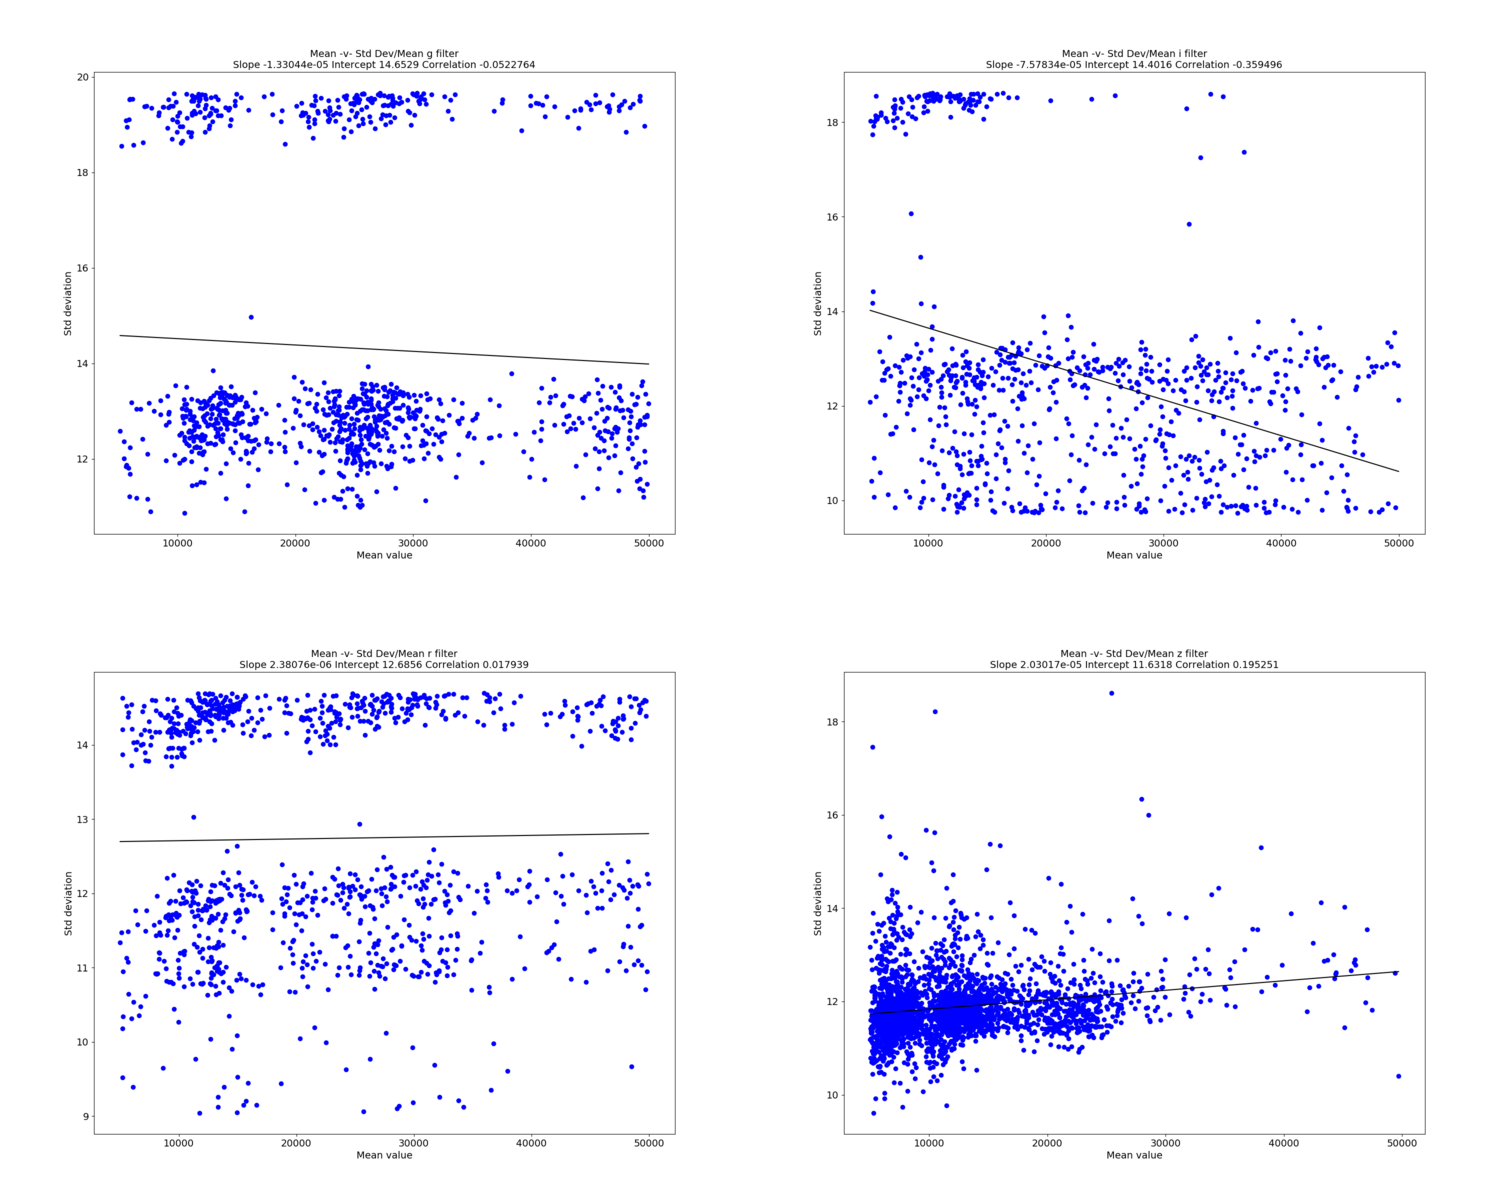
\includegraphics[scale=0.25]{images/Corr.png} \\
\end{center}   
\caption{This figure shows how the standard deviation of the values in the
daily flat files corresponds to the four filters. In the top is shown the
results for the \texttt{g} filter, the bottom left shows the \texttt{r} filter,
the top right shows the results for the \texttt{i} filter and the bottow right
shows the results for the \texttt{z} filter. The black line shows the best fit
slope in each case.}
\protect\label{fig:ffcorr}
\end{figure}

\subsubsection{Display of flat filesl}

A profile of the master flat files was taken by ``slicing'' throuh rows and
columns. In Fig. \ref{fig:mbyrow} are shown 4 rows and the column value in a master flat file (for September 2019) and the
by columns in Fig. \ref{fig:mbycol}.

\begin{figure}[!htbp]
\begin{center}
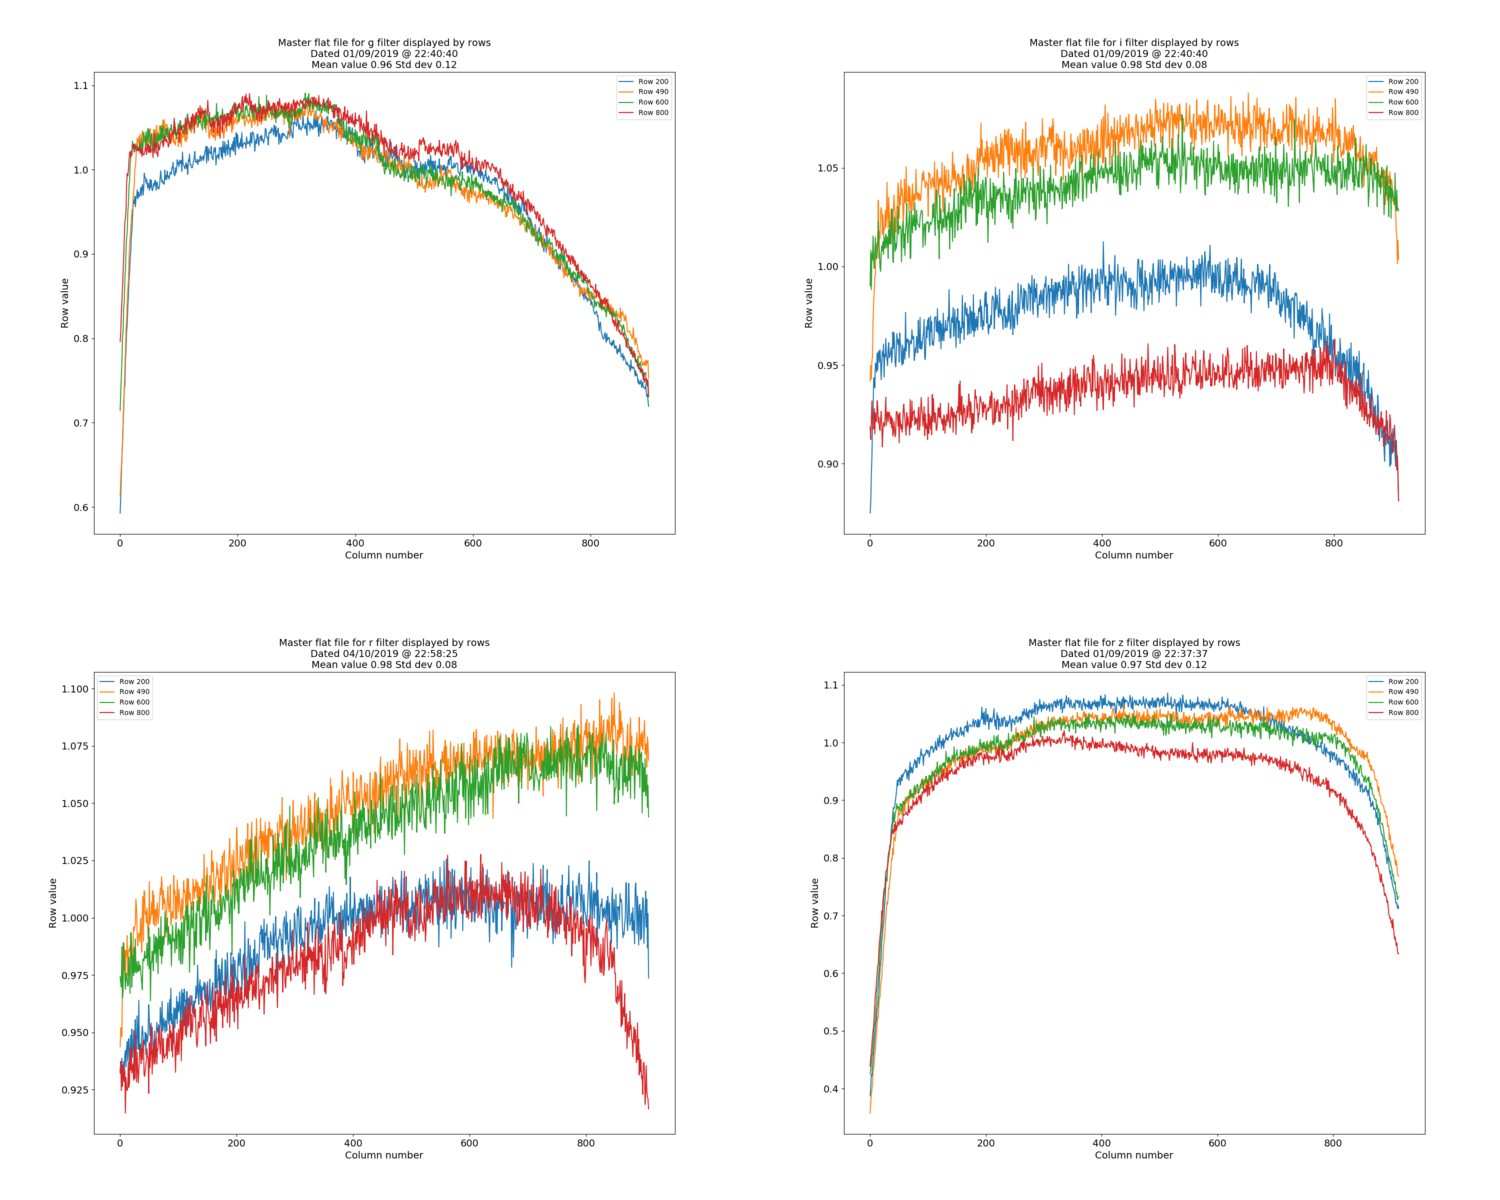
\includegraphics[scale=0.25]{images/Cmrowd.png} \\
\end{center}   
\caption{This figure shows the pixel values in the master flat files for the
four filters for the month of September 2019, selecting rows 200, 400, 600 and
800 in the file.
In the top is shown the results for the \texttt{g} filter, the bottom left shows the \texttt{r} filter,
the top right shows the results for the \texttt{i} filter and the bottow right
shows the results for the \texttt{z} filter. }
\protect\label{fig:mbyrow}
\end{figure}

\begin{figure}[!htbp]
\begin{center}
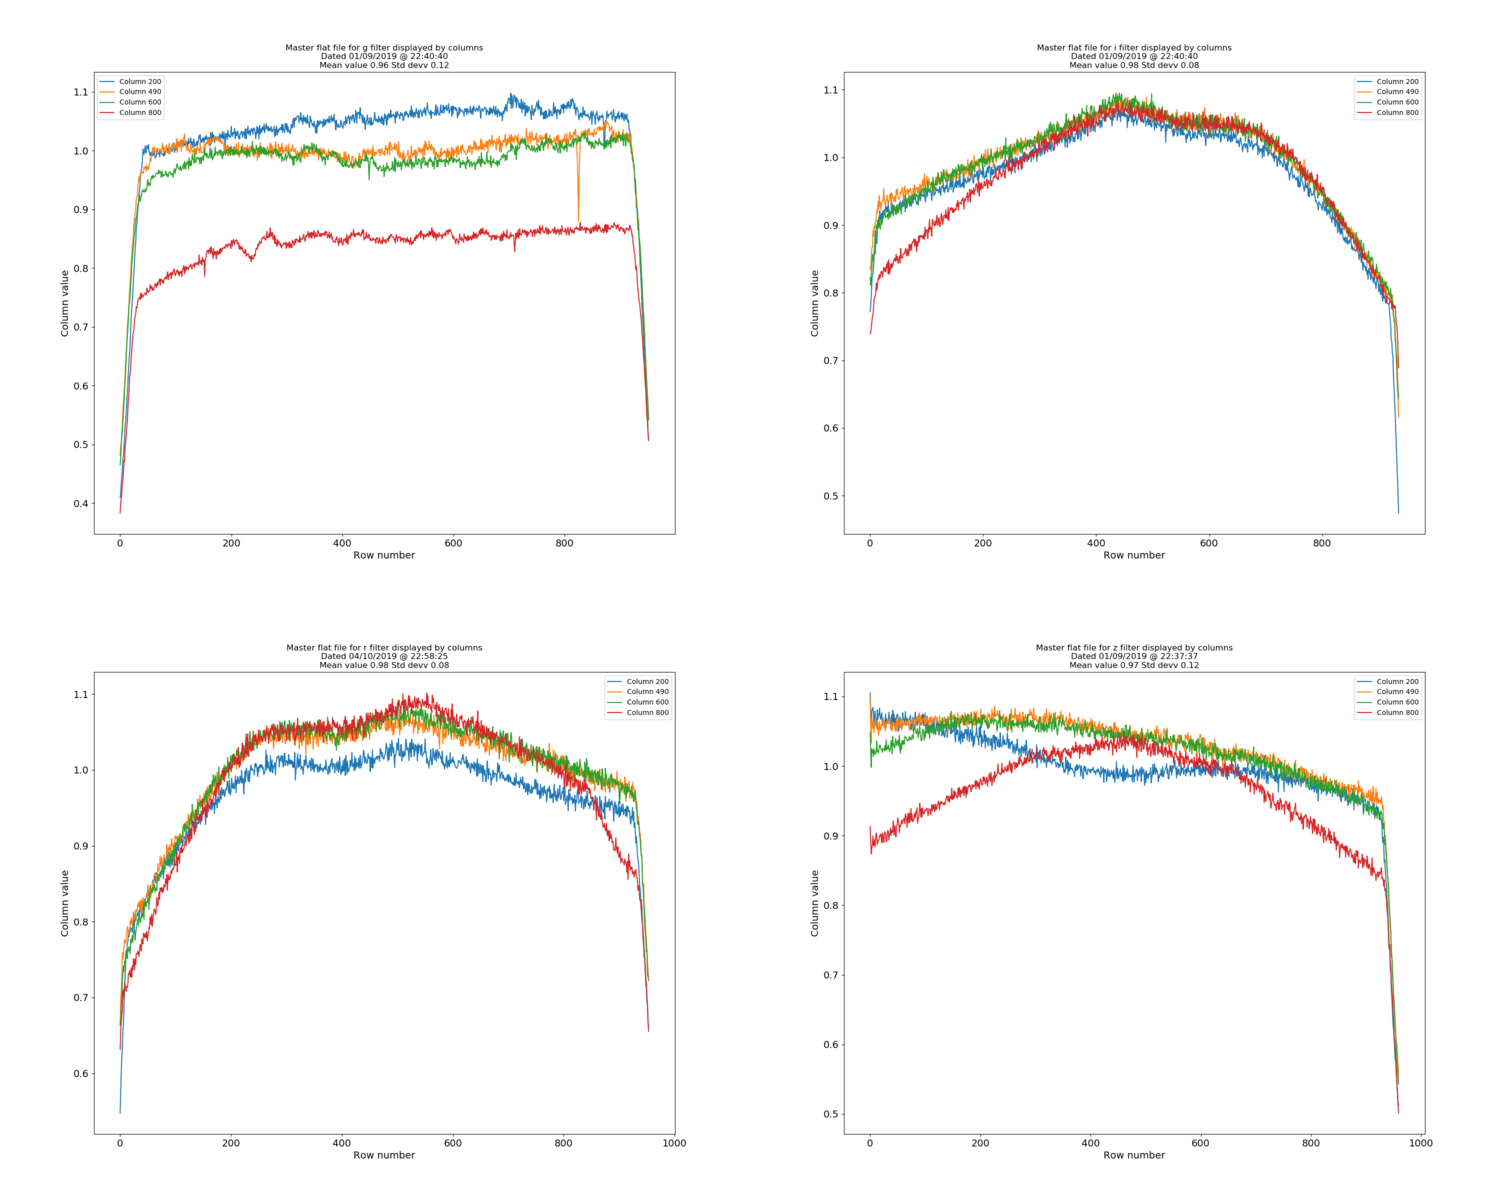
\includegraphics[scale=0.25]{images/Cmcold.png} \\
\end{center}   
\caption{This figure shows the pixel values in the master flat files for the
four filters for the month of September 2019, selecting columns 200, 400, 600
and 800 in the file.
In the top is shown the results for the \texttt{g} filter, the bottom left shows the \texttt{r} filter,
the top right shows the results for the \texttt{i} filter and the bottow right
shows the results for the \texttt{z} filter. }
\protect\label{fig:mbycol}
\end{figure}
\clearpage

The daily flat files which were selected, i.e.mean values between 5,000 and
50,000 counts, took a similar profile.

\subsection{Bias files}
\protect\label{section:biasfiles}

As with the flat files, daily and monthly master bias files are saved. However
the master bias files are stored as integer pixels, presumably an average of the
daily bias files. The master bias files, unlike the master flat files, do not
include any indication of which daily bias files go into their construction.

In the treatment of the bias files herein, the images are trimmed by removing
rows and columns which contain \texttt{NaN} in the corresponding monthly master
flat file.

As discussed in Section \ref{section:tdataprovided} The images were processed according to the formula:

\begin{center}
$ \frac{(mage - bias) \times mf}{flat - bias}$
\end{center}

In this $mf$ represents to mean value of the flat pixels, which was supposed to
be normalised to be 1 in the master flat files. In fact it is not. The master
flat files are advertised to have the bias already subtracted.

It was noticed that in some cases the calculation above gave negative results,
i.e. the bias values in some pixels were greater than the corresponding ones in
the images. For example, taking the observations and master bias files for 5
September 2018, the total negative values shown in Table \ref{table:negmast} are
observed.

\begin{table}[!htbp]
\begin{center}
\begin{tabular}{lrr} \hline
Filter & Min & \% negative \\\hline
g & -27 & 28.90 \\
i & -20 & 5.42 \\
r & -19 & 5.52 \\
z & -20 & 9.90 \\
\hline
\end{tabular}
\end{center}
\caption{Negative values of pixels in image minus monthly master bias for
various filters on 5 September 2018, for all observations of \bstar, through
various visible light filters}.
\protect\label{table:negmast}
\end{table}

It is noticeable that this is worst on the \texttt{g} filter, for which some of
the best results were obtained finding images. An example of the distribution of
negative values after subtracting the appropriate master bias from the sky is
shown in Fig.
\ref{fig:negbiaseg}

\begin{figure}[!htbp]
\begin{center}
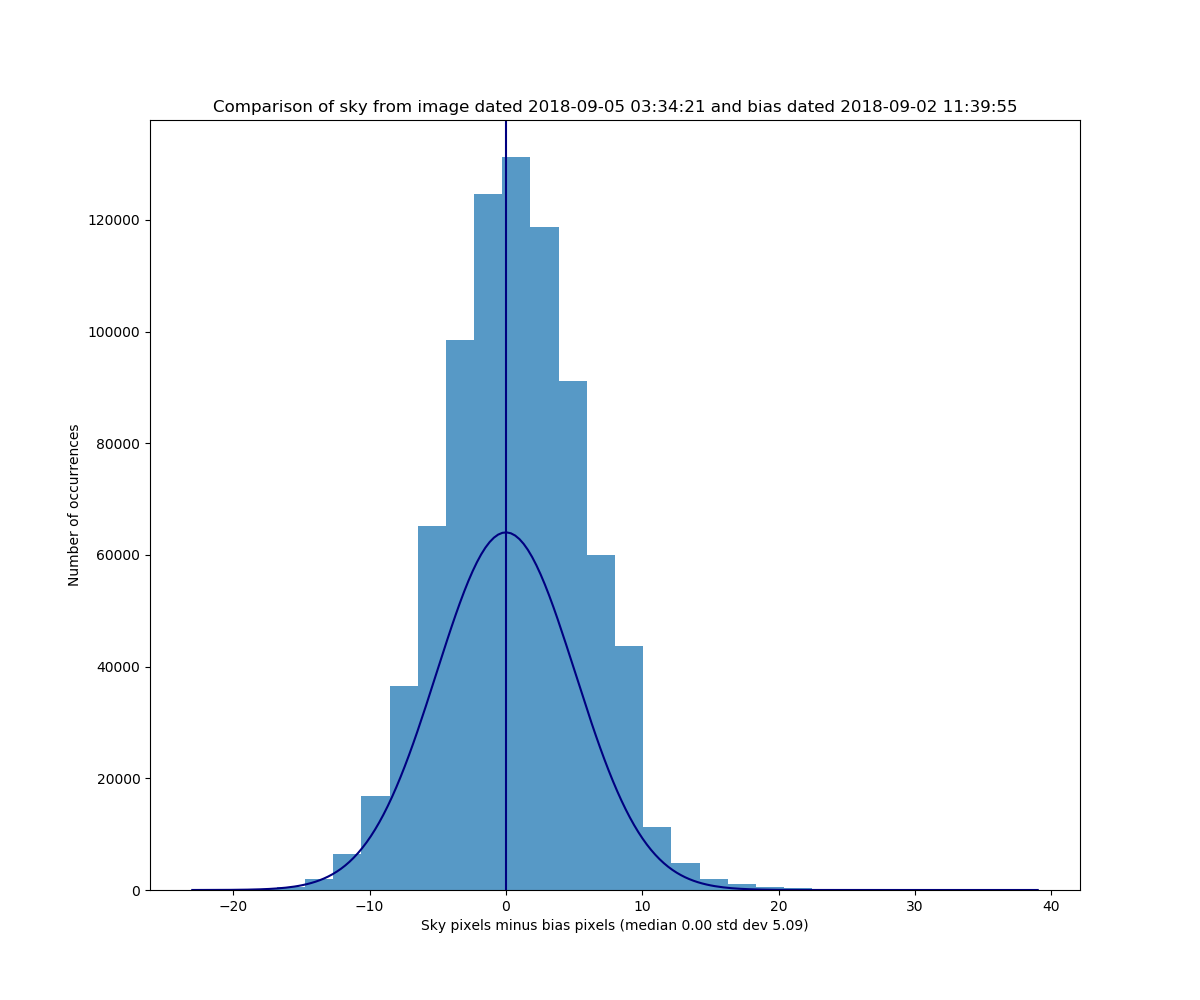
\includegraphics[scale=0.5]{images/negbiaseg.png}
\end{center}   
\caption{This shows the distribution of the values of the sky level pixels minus
the corresponding bias pixels for an observation of {\bstar} with the \texttt{g}
filter taken on on 5 September 2018 and the master bias file for September 2018.}
\protect\label{fig:negbiaseg}
\end{figure}

\subsubsection{Comparison of bias files}

The master bias files are constructed from daily bias files and it seemed
appropriate to examine these. on 5 September 2018, five daily bias files were
taken between 11:31:10 UTC and 11:37:02 UTC for each filter.

Each consecutive pair of bias files were compared against each other (after
eliminating ``spikes'' from cosmic rays) and the results set out in Fig.
\ref{fig:biascomp}.

\begin{figure}[!htbp]
\begin{center}
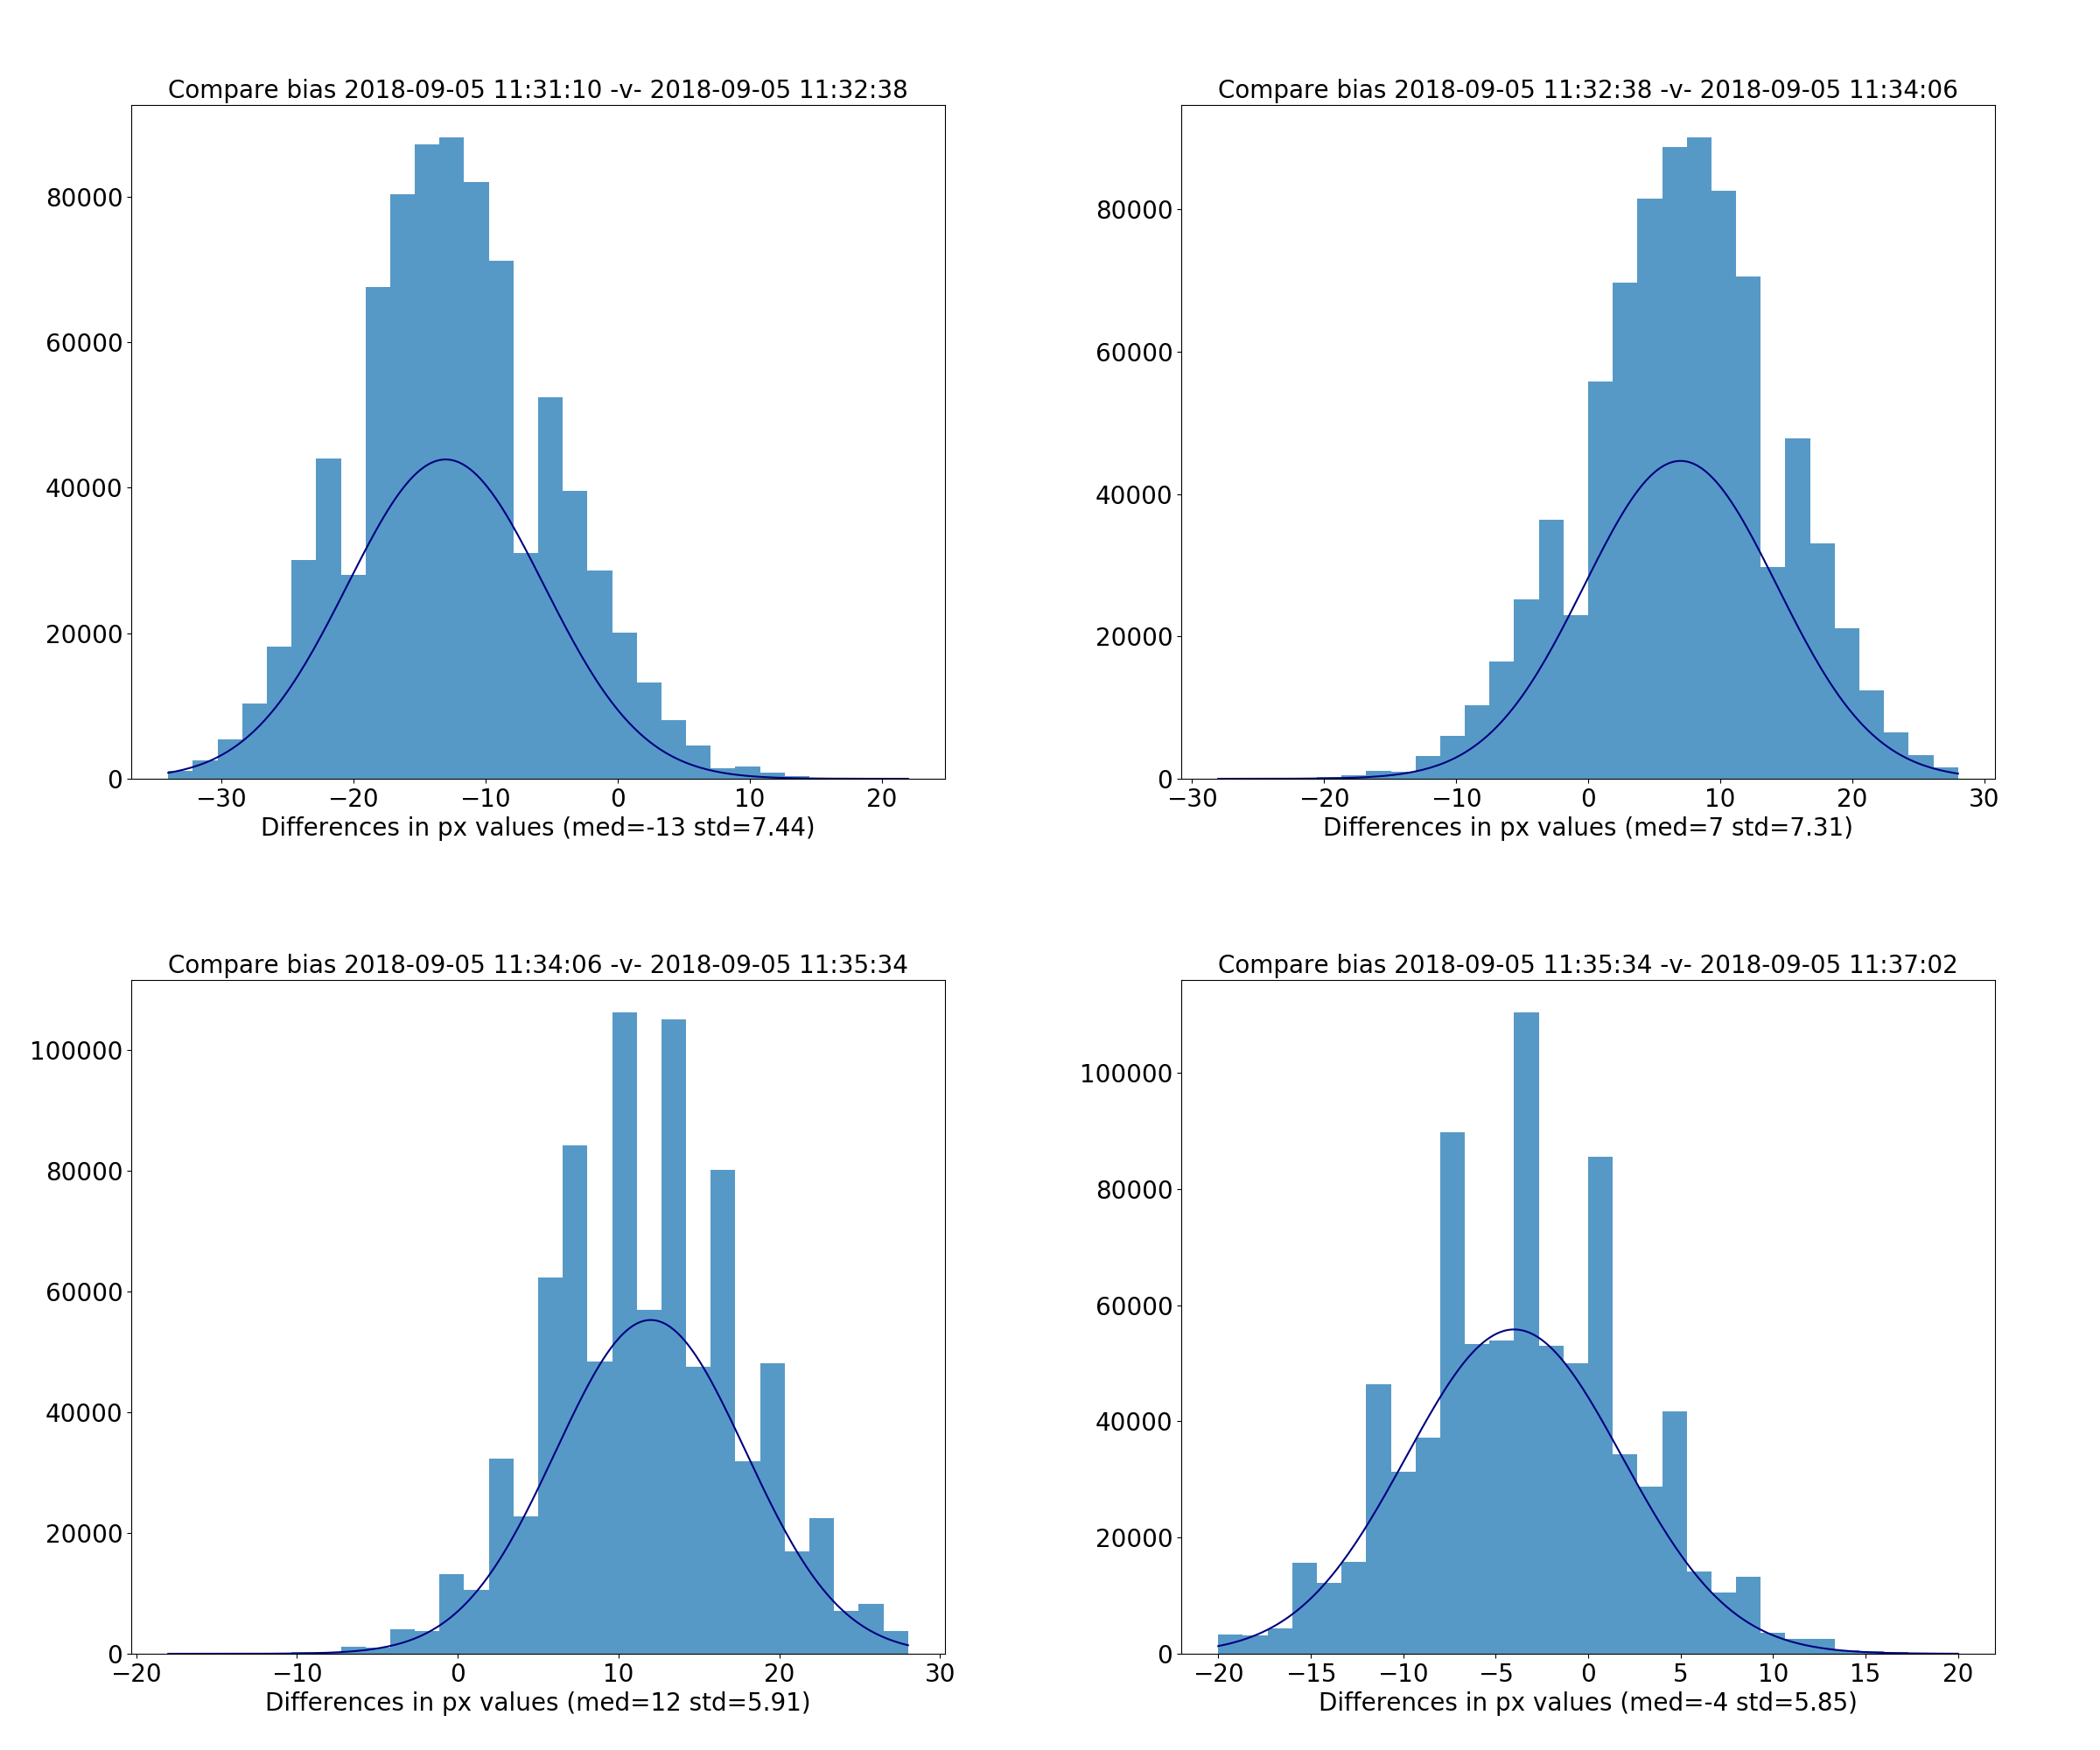
\includegraphics[scale=0.2]{images/biascomp.png}
\end{center}   
\caption{This shows the differences between successive pairs of the 5 bias
files taken on 5 September for filter \texttt{g} with times as shown in the
titles between 11:31:10 UTC and 11:37:02 UTC} \protect\label{fig:biascomp}
\end{figure}

Similar results were observed when bias files for other filters were observed,
for other dates and daily bias files several days apart were compared. The
differences would appear to be a measure of the errors in the CCD used.

A bias file was constructed by merging together all the daily bias files and the
computation shown in Fig. \ref{fig:negbiaseg} for the monthly master
bias file repeated, the result is very similar, as shown in Fig.
\ref{fig:negbiasmerg}.

\begin{figure}[!htbp]
\begin{center}
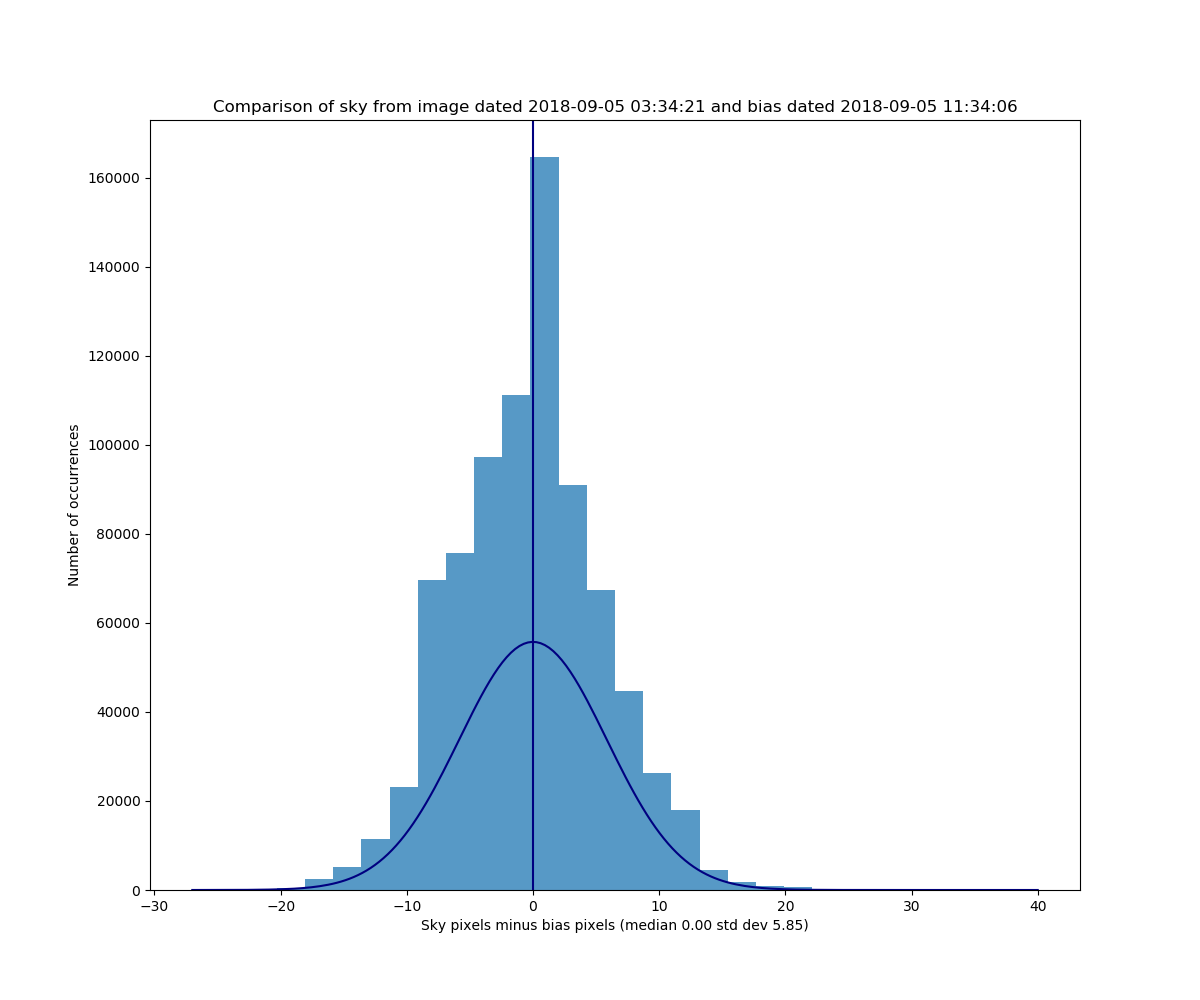
\includegraphics[scale=0.5]{images/negbiasmerg.png}
\end{center}   
\caption{This shows the distribution of the values of the sky level pixels minus
the corresponding bias pixels for an observation of {\bstar} with the \texttt{g}
filter taken on on 5 September 2018 and a bias file constructed from the bias
files taken on 5 September 2018.} \protect\label{fig:negbiasmerg}
\end{figure}

It was noticeable that, except in the case of images which were clearly
defective in other ways, the difference between the merged bias levels and the
sky levels was at most that of the standard deviation between the bias levels
shown in Fig. \ref{fig:biascomp} and was often zero as Fig.
\ref{fig:negbiaseg} and Fig. \ref{fig:negbiasmerg} show. This would suggest that
the bulk of the ``sky level'' is made up of the bias values.

\subsubsection{Accuracy}
Combination of daily bias values appears to improve the accuracy. The median
pixel value for all of the bias files for all of the filters is approxiamtely
300 with a standard deviation of about 7 for the individual files, 3 for where
all the daily ones for a given day are merged and 1 for the master bias files.

If the counts on the actual images are considered, the following maximum pixel
values are observed, as illustrated in Table \ref{table:pmaxima}. Note that
these are extreme cases. The typical maximum is about 75\% of these.

The values displayed are in all cases for the target object, \bstar. Reference
objects which are ``found'' have ADUs about 25\% of those figures, whist other
objects only just discernible on the images but not ``found'' by the algorithm
have maximum ADUs of about 450.

\begin{table}[!htbp]
\begin{center}
\begin{tabular}{lr} \hline
Filter & Max pixel value \\\hline
g & 5,010 \\
i & 56,509 \\
r & 16,562 \\
z & 34,293 \\
\hline
\end{tabular}
\end{center}
\caption{Maximum pixel values in any of the observation files for 5 September
2018.}.
\protect\label{table:pmaxima}
\end{table}
\clearpage

% \subsection{Analysis of images}
% \protect\label{section:analimages}
% 
% \textbf{Please note that since I realised that the master flat files are not
% normalised as Luciano told me I'll have to redo all this. The results within
% each month are consistent but not with other months. Also with the flat files
% properly normalised some of the images will have greater contrast.}
% 
% \subsubsection{Intensity comparison}
% \protect\label{section:intcomp}
% 
% As a first attempt to study the data, the ADU count was taken, specifically the
% net after applying the flat and bias files of the target in all the images in which it was available.
% The target was found in all of the images, apart from in a few of the
% \textbf{g}, \textbf{i} and \textbf{r} visible light filters,
%, as shown in Table
%\ref{table:occtb} below.

%Plotting light curves of the intensities obtained in this way yields Fig.
% \ref{fig:allall}.
%Binning the intensities together into a single day gave
%Fig. \ref{fig:allbin}, the error bars indicate the spread over a single day.

%I plotted
%periodograms, as shown in Fig. \ref{fig:pgrams}. Despite the crudeness of the
%data, it is noticeable that there are peaks close to the rotation periods of
% the order of 150 days referred to in \citet{suarezmascareno15} and \citet{toledopadron18}.

% \begin{figure}[!htbp]
% \begin{center}
% 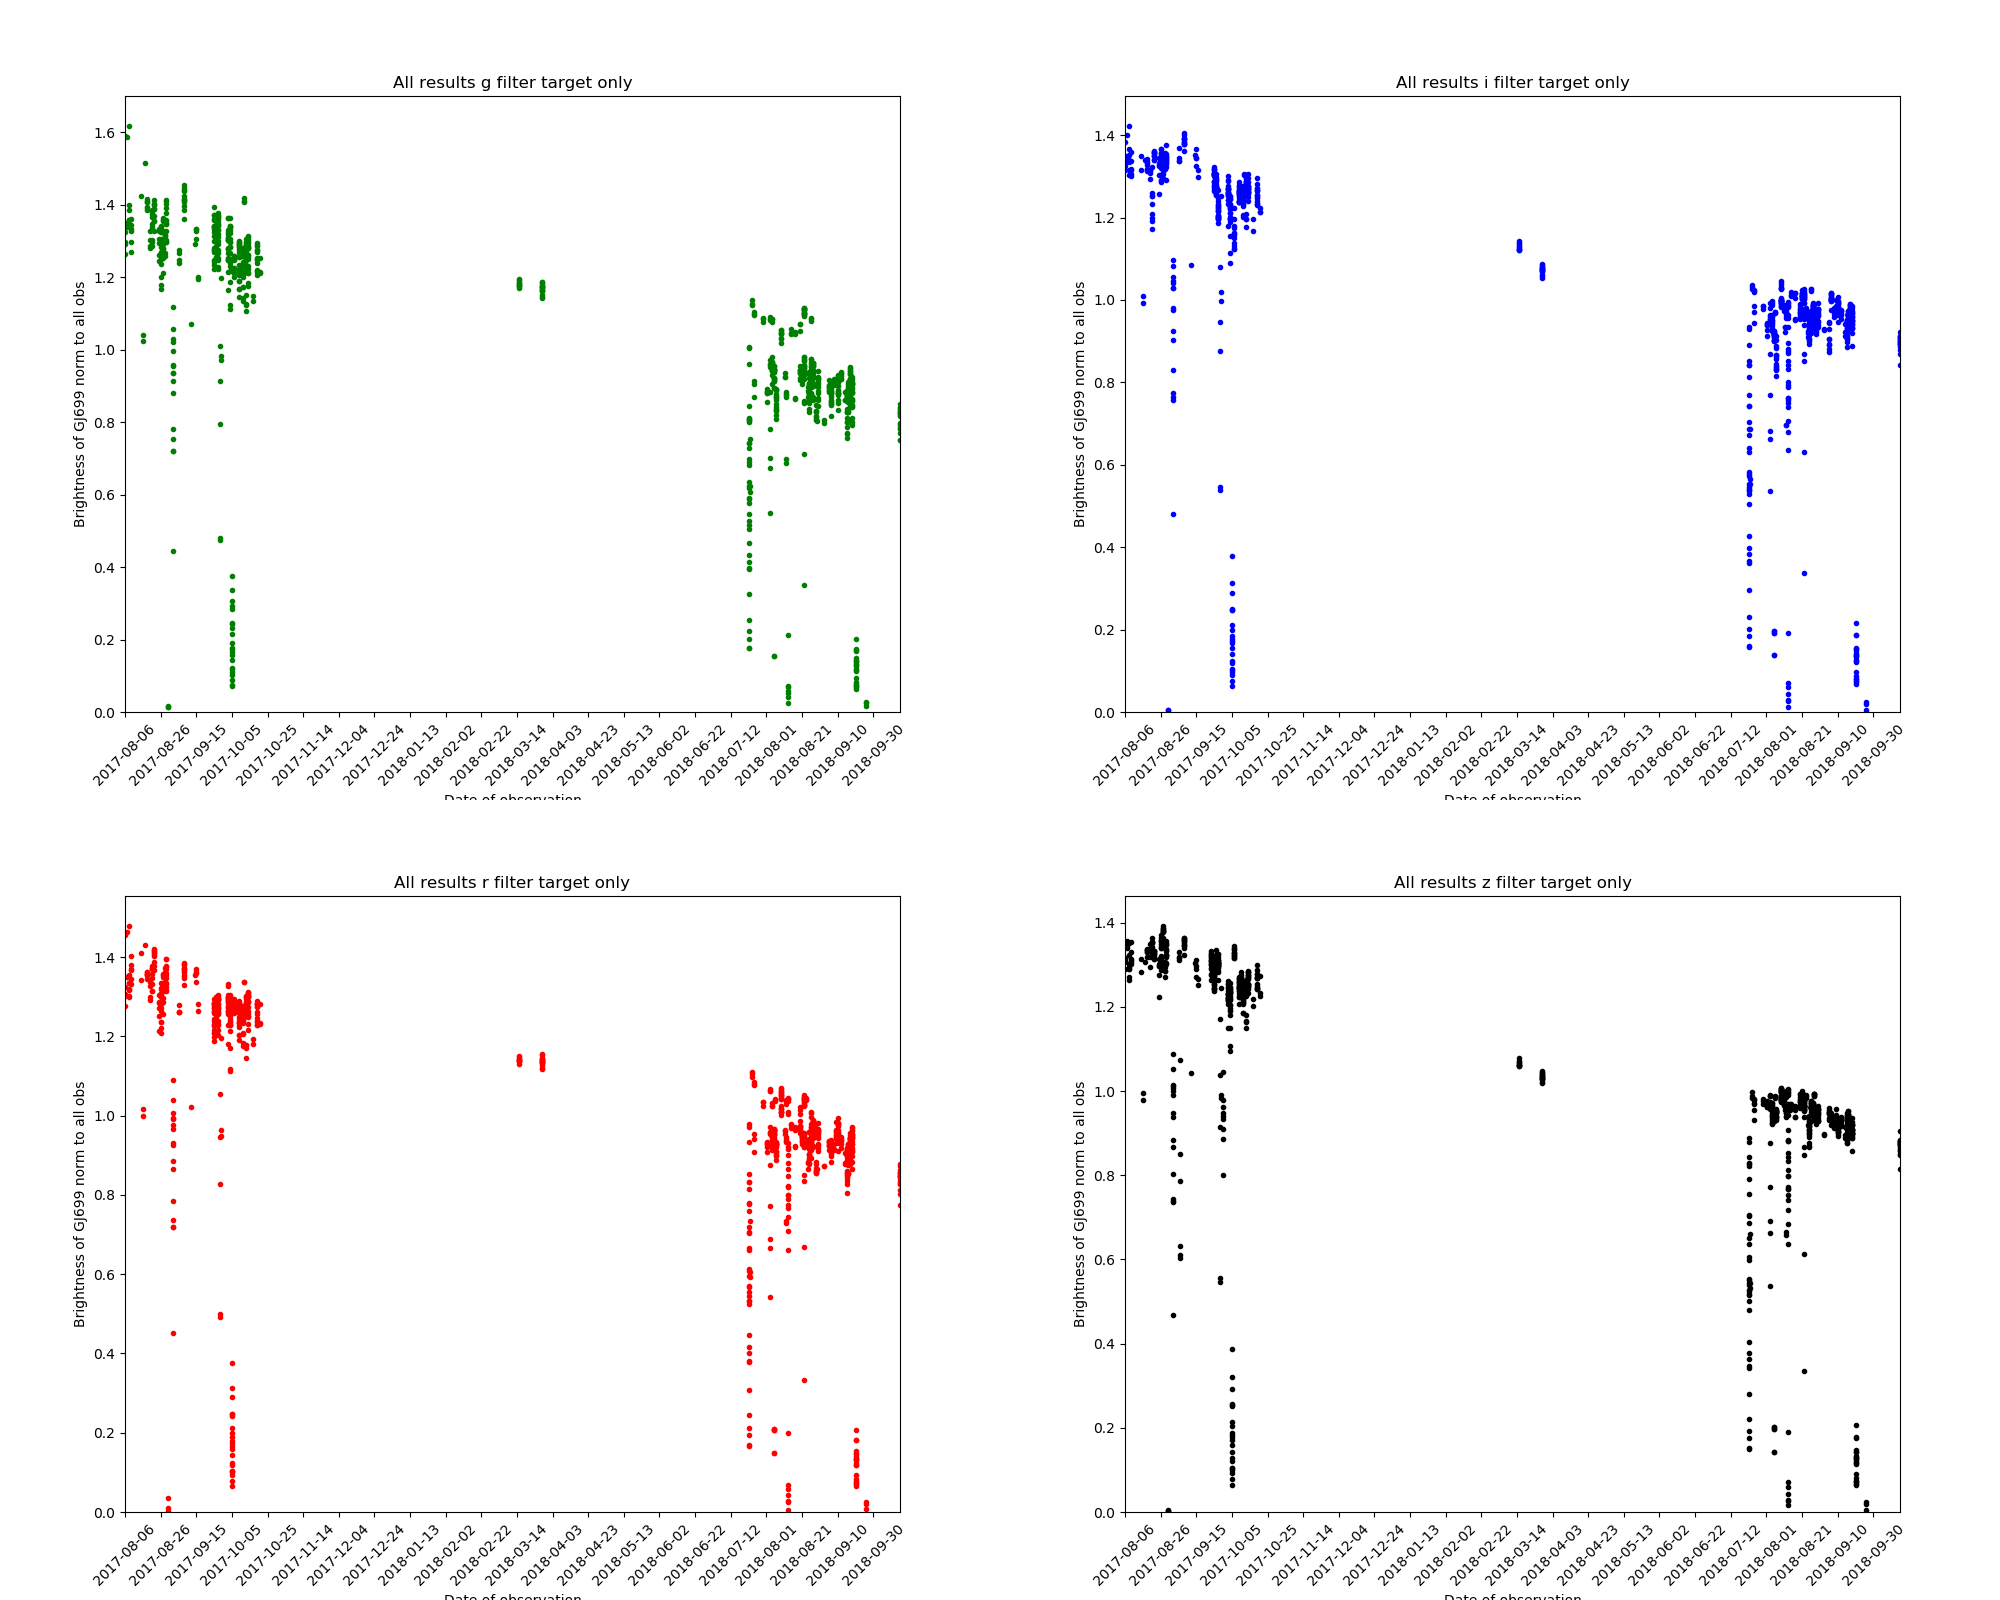
\includegraphics[scale=0.25]{images/allall.png} \\
% \end{center}   
% \caption{This shows the flux for the target, \bstar, for each of the four visible light filters. This takes the total
%   ADU count only}
%   \protect\label{fig:allall}
% \end{figure}
% 
% \begin{figure}[!htbp]
% \begin{center}
% 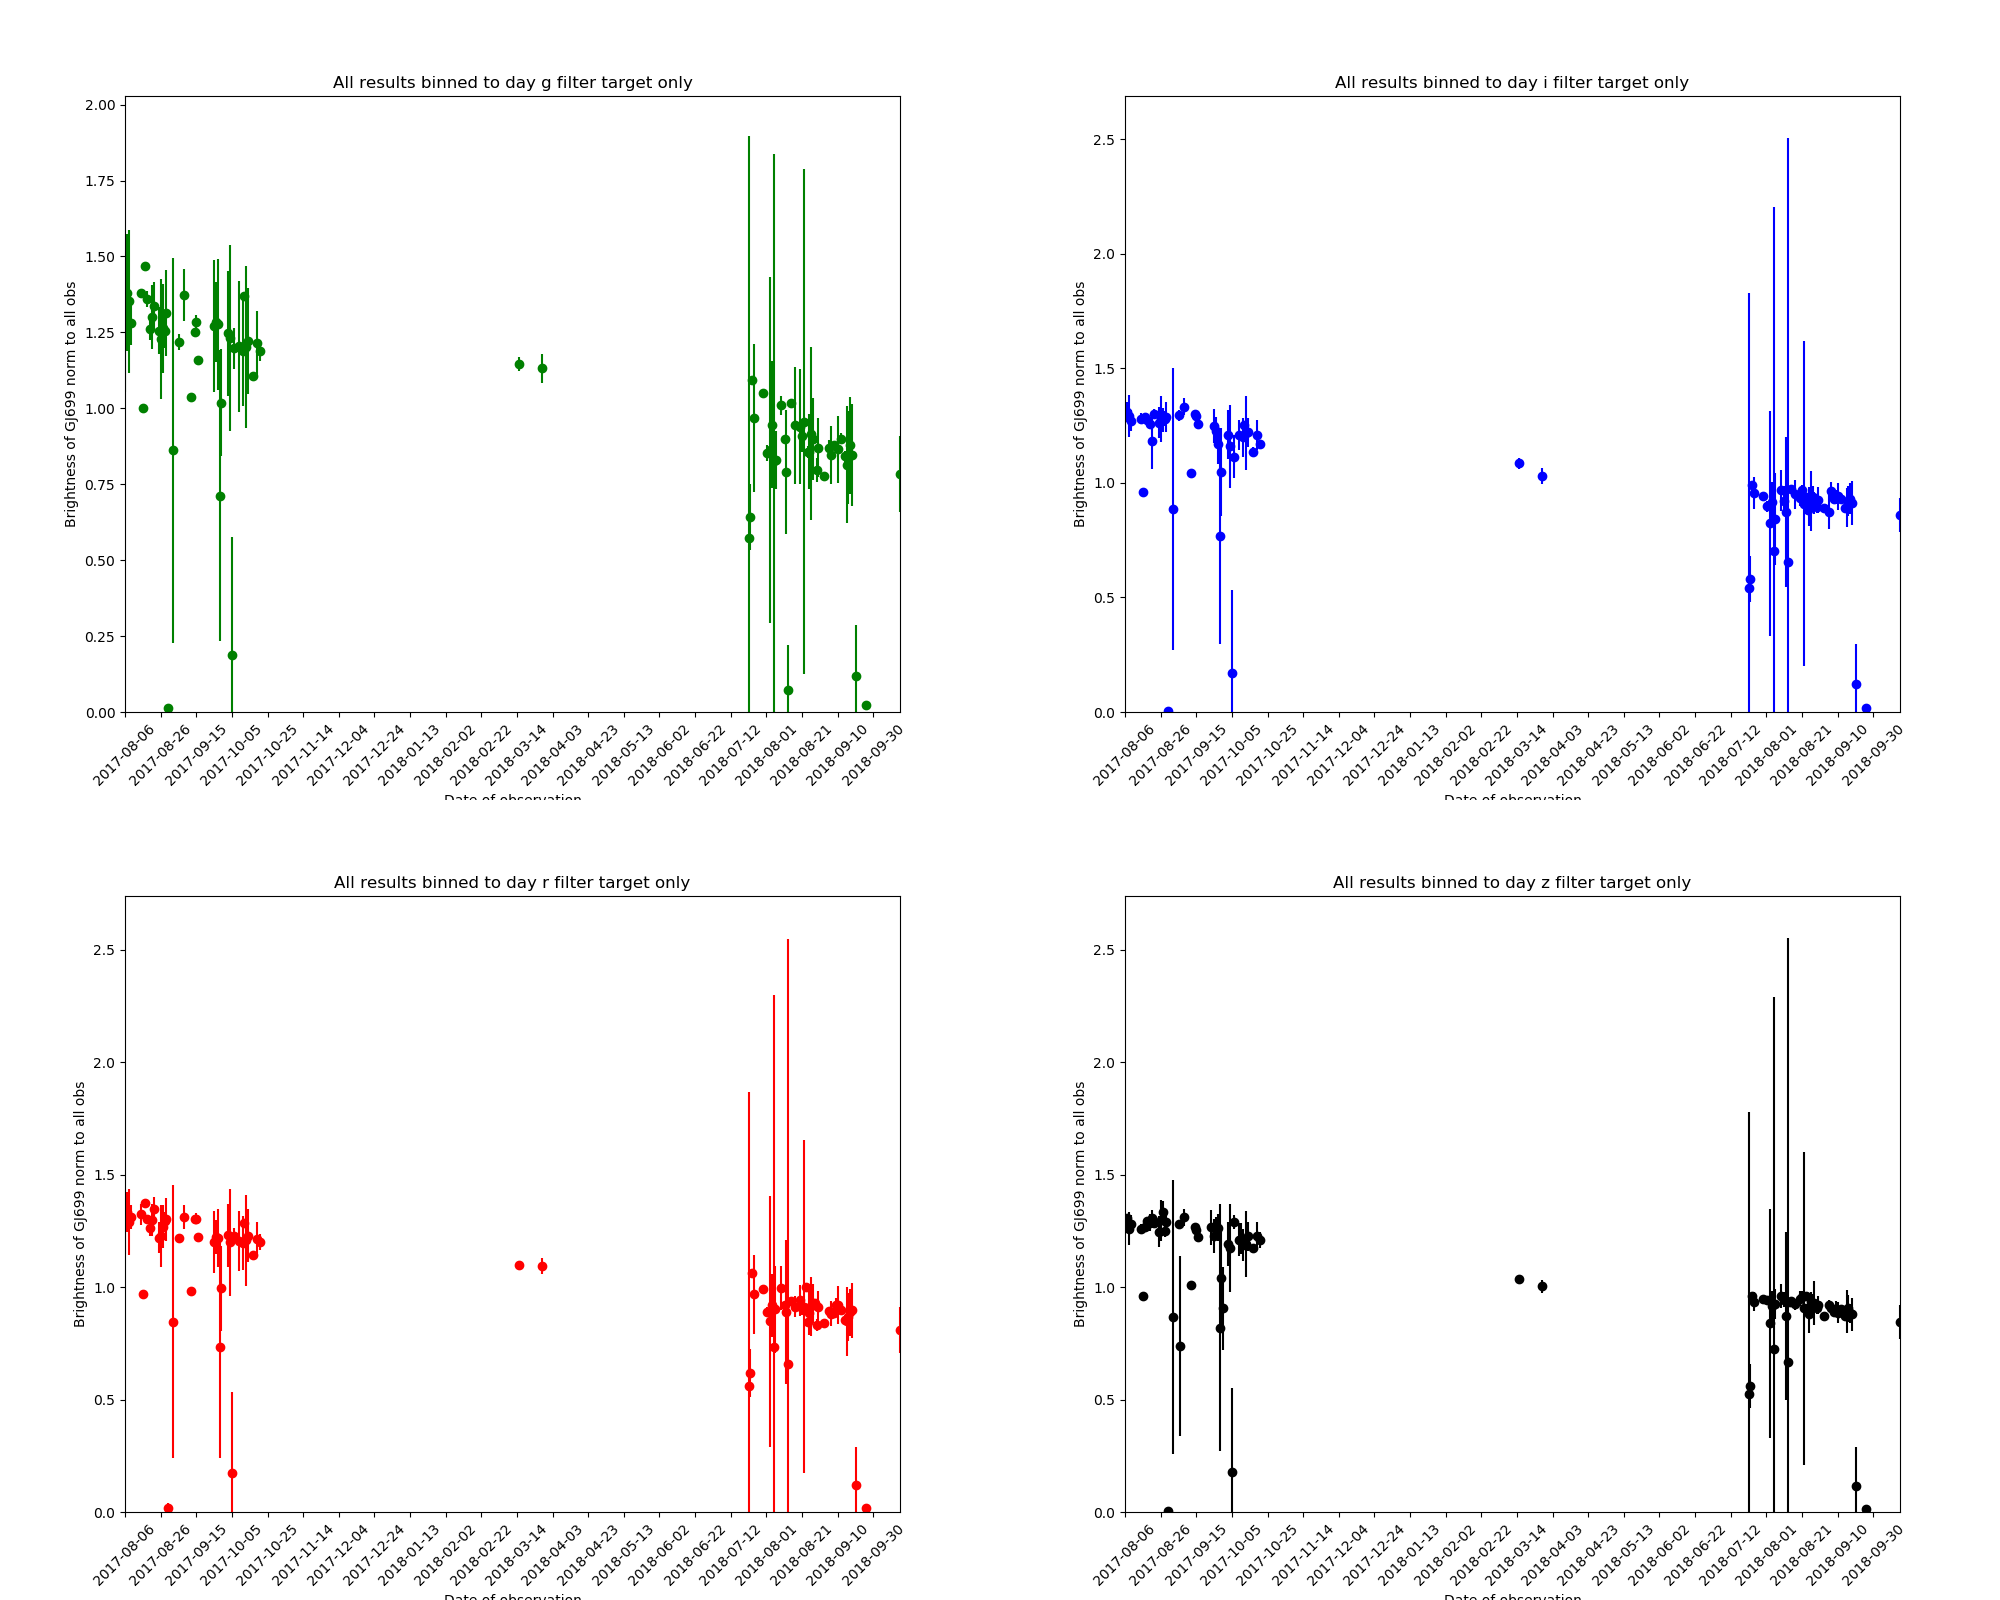
\includegraphics[scale=0.25]{images/allbin.png} \\
% \end{center}   
% \caption{This shows the flux for the target, \bstar, for each of the four visible light filters and binned to a single day. Error bars are show to indicate the spread of intensities over a single day.}
%   \protect\label{fig:allbin}
% \end{figure}

%\begin{figure}[!htbp]
%\begin{center}
%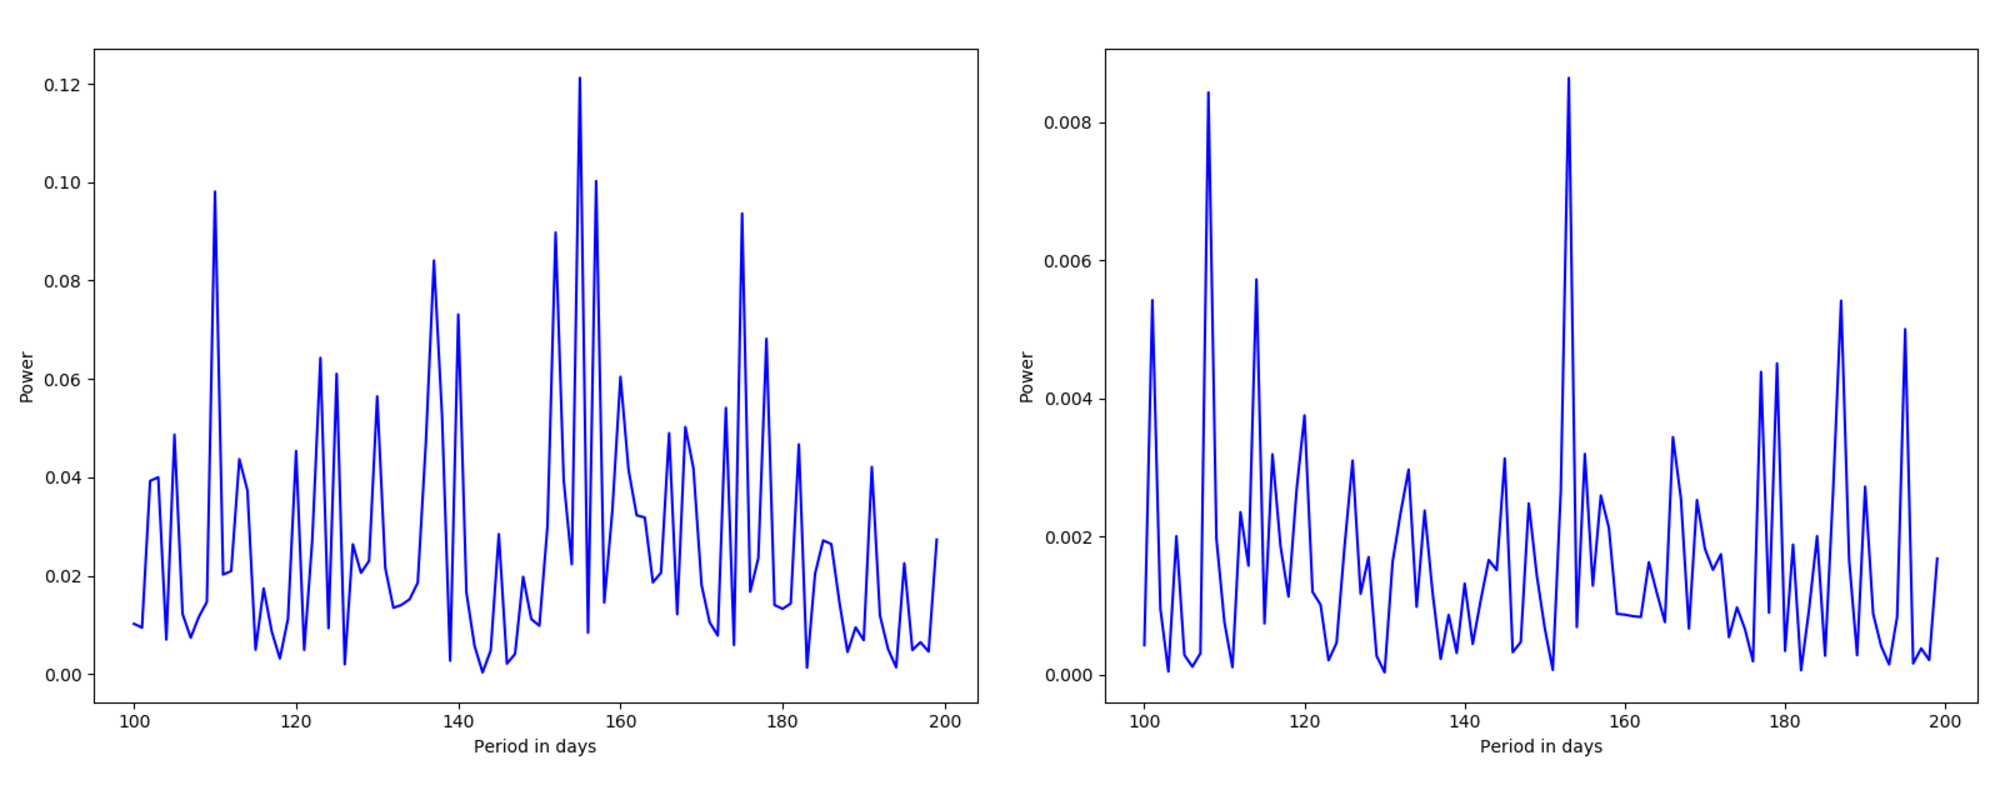
\includegraphics[scale=0.25]{images/pgrambunb.png} \\
%\end{center}   
%\caption{This displays periodograms derived from the binned (Fig.
% \ref{fig:allbin}) and unbinned (Fig. \ref{fig:allall}) light curves for the \textbf{r} filter.}
%  \protect\label{fig:pgrams}
%\end{figure}

% It is accepted that this initial treatment is crude. Serious work needs to be done on correction for air mass,
% which for a few observations, where they are spread over a period of several hours,
% can be quite large, and to more accurately discard as unacceptable images with large or very variable sky levels.
% There are some currently inexplicable variations, for
% example the to images in Fig. \ref{fig:tyeg} give radically different ADU counts despite being taken two minutes apart
% with same exposure time and other parameters.
% 
% \begin{figure}[!htbp]
% \begin{center}
% 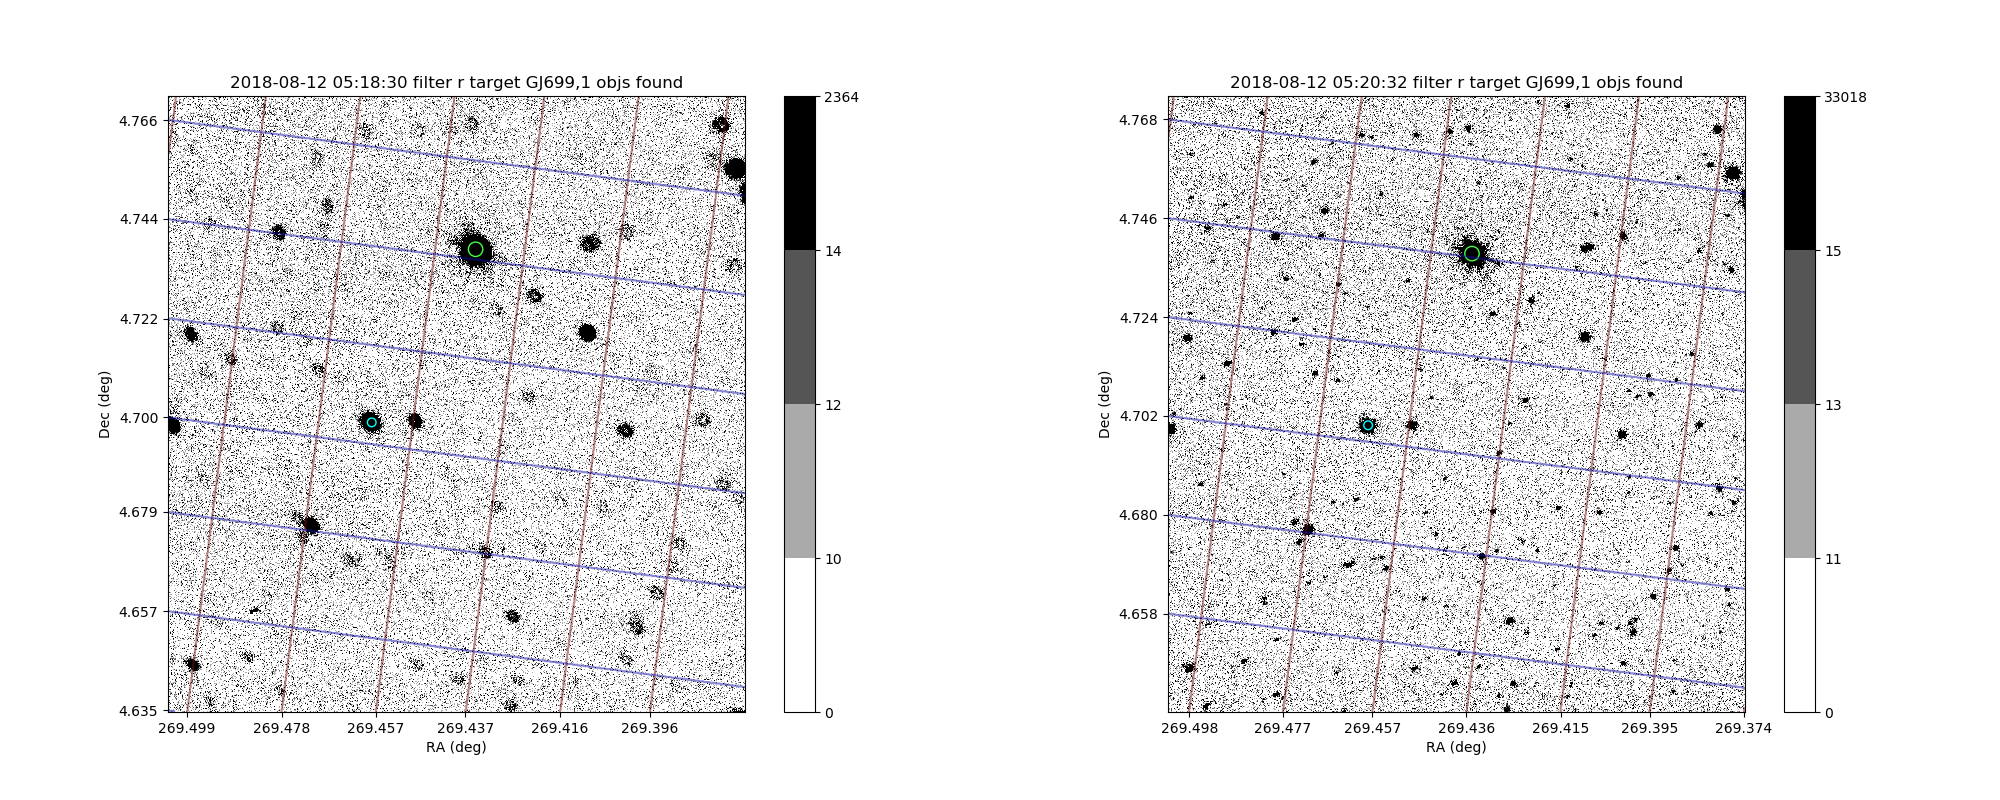
\includegraphics[scale=0.25]{images/tyeg.png}
% \end{center}   
% \caption{These images show an example of where 2 images taken 2 minutes apart with the same exposure time gave different flux values.}
%   \protect\label{fig:tyeg}
% \end{figure}
% 
% \subsubsection{Reference Stars}
% \protect\label{section:refstars}
% 
% Rather than relying on the ``raw'' flux from the target star itself, it was
% considered that an approach based on identified reference stars found in a
% significant number of images.
% Ideally these should be as many as possible to ``smooth'' out errors and variations on the reference star. 
% Byy taking the ratio of the target star ADU count to the sum of the reference
% star ADUs, then we can hope to achieve results for intensity with the factors such air mass corrections factored out, This
% approach was taken in \citet{berry11} and would seem to involve least work, provided sufficient reference stars are
% consistently found.
% 
% The algoritm used to find objects was first to locate the target (there was
% usually a certain amount of error in the coordinates of the images) and then
% find prefeviously-known reference objects. The criterion for finding objects was to look for groups of pixels within a
% given scan aperture whose mean count was a given number of standard deviations
% (intially 3) from that of the sky level. If the result appeared to be one of
% the objects known already, the given reference object was deemed to have been
% found.

% In all cases the brightest objects were found in Simbad, 2MASS and SDSS
% to find objects in the vicinity of \bstar, obtaining the following stars as shown in Table \ref{table:reftimesfound}.
% Of the stars there, the types are unavailable apart from the most-frequently occurring one of
% TYC425-262-1, which is an A3V star (this is also reported as the most frequently found reference star in \citet{berry11}).
% 
% \begin{table}[!htbp]
% \begin{center}
% \begin{tabular}{llr} \hline
% Number & Object & Times found \\\hline
% 1 & TYC425-262-1 & 5,277 \\
% 2 & SDSS1237671695527248969 & 3,408 \\
% 3 & 2MASSJ17574653+0447466 & 3,297 \\
% 4 & SDSS1237668573088841773 & 840 \\
% 5 & TYC425-223-1 & 369 \\
% 6 & SDSS1237671695527249415 & 15 \\
% \hline
% \end{tabular}
% \end{center}
% \caption{This lists the identified reference objects near to {\bstar} and the number of times found in the available
%   data. Note that this data relates to images up to the end of October 2018.}
% \protect\label{table:reftimesfound}
% \end{table}
% 
% I decided to consider only the first 3 reference objects, which are labelled 1, 2 and 3 for convenience in the
% remainder of this report, as the appearances of the others were too infrequent to render them worthwhile.
% 
% \subsection{Classification of results}
% \protect\label{section:classresults}
% 
% The images presented challenges in various respects. The visible light images are all at different orientations and with
% the target in different places in the image, so not all the reference stars appear in all of the images. In some cases
% the reference stars are just not bright enough to rise sufficiently above the sky level.
% 
% \begin{table}[!htbp]
% \begin{center}
% \begin{tabular}{lrrrr}
% &Filter g&Filter i&Filter r&Filter z\\\hline
% Target not found&167&80&105&0\\
% No ref objs found & 84 & 1,003 & 53 & 1,085 \\\hline
% Obj 1 (with or without others) & 834 & 0 & 925 & 0 \\
% Obj 2 (with or without others) & 561 & 1 & 574 & 0 \\
% Obj 3 (with or without others& 526 & 0 & 573 & 0 \\
% Obj 1 only & 43 & 0 & 100 & 0 \\
% Obj 2 only & 0 & 1 & 1 & 0 \\
% Obj 3 only & 0 & 0 & 0 & 0 \\
% Objs 1 and 2 (with or without 3) & 561 & 0 & 573 & 0 \\
% Objs 1 and 3 (with or without 2) & 526 & 0 & 573 & 0 \\
% Objs 2 and 3 (with or without 1) & 296 & 0 & 321 & 0 \\
% Objs 1 and 2 only & 265 & 0 & 252 & 0 \\
% Objs 1 and 3 only & 230 & 0 & 252 & 0 \\
% Objs 2 and 3 only & 0 & 0 & 0 & 0 \\
% Objs 1,2 and 3 & 296 & 0 & 321 & 0 \\
% \hline
% \end{tabular}
% \end{center}
% \caption{This table shows the occurrences of the 3 main reference objects in each of the observations with or without
%   the others. The infrared images were omitted as no reference objects were found in any of them. Note however the lack
%   of occurrences of reference objects in the \textbf{i} and \textbf{z} filter images.}
% \protect\label{table:occtb}
% \end{table}
% 
% \subsection{Results from reference object comparisons}
% \protect\label{section:refobjres}
% 
% Repeating the light curve plots from Section \ref{section:intcomp}, this time as the ratio of the ADU count of the
% target to the sum of the first three reference objects, Fig.  \ref{fig:allref123} and Fig. \ref{fig:allref123bin} show
% the light curves for the \textbf{r} and \textbf{g} filters. Also shown in Fig. \ref{fig:ls123both} are periodograms
% derived from these light curves. Also shown in Fig \ref{fig:allref1}, Fig. \ref{fig:allref1bin} and Fig. \ref{fig:ls1both}
% are the corresponding results taking into account only the brightest of the reference objects, TYC425-262-1.
% 
% \begin{figure}[!htbp]
% \begin{center}
% 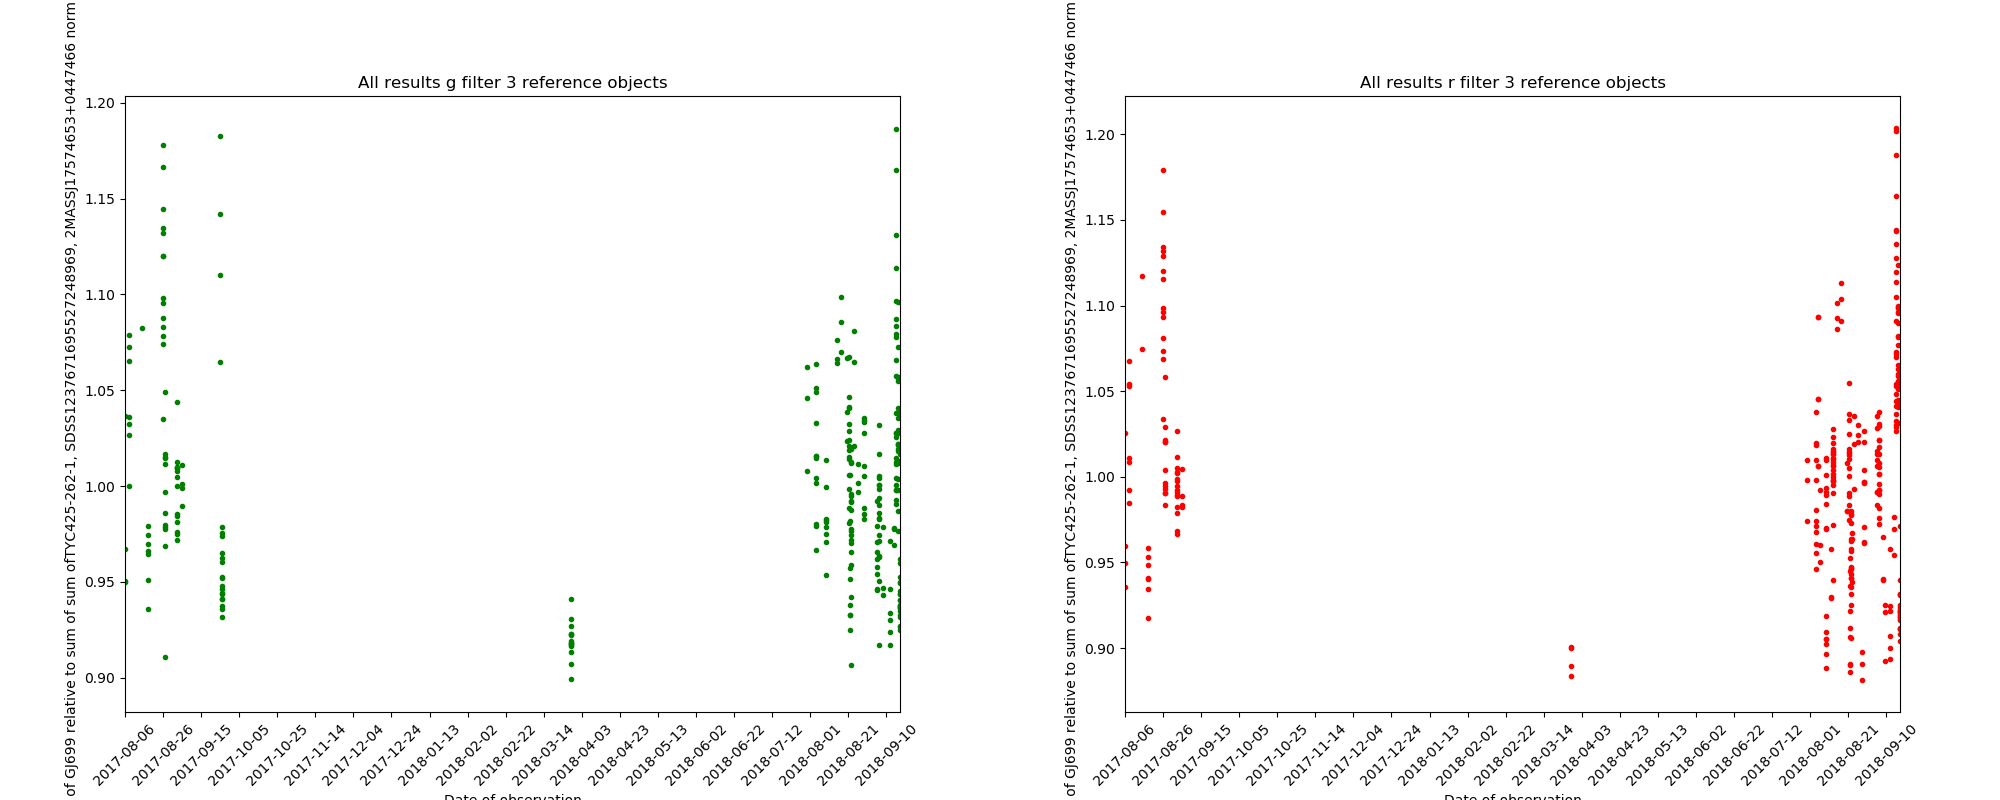
\includegraphics[scale=0.25]{images/allref123.png}
% \end{center}   
% \caption{This shows the ratio of the flux for the target, \bstar, to the 3 main reference objects for the \textbf{g} and
% \textbf{r} filters, plotted as green and red respectively.}
%   \protect\label{fig:allref123}
% \end{figure}
% 
% \begin{figure}[!htbp]
% \begin{center}
% 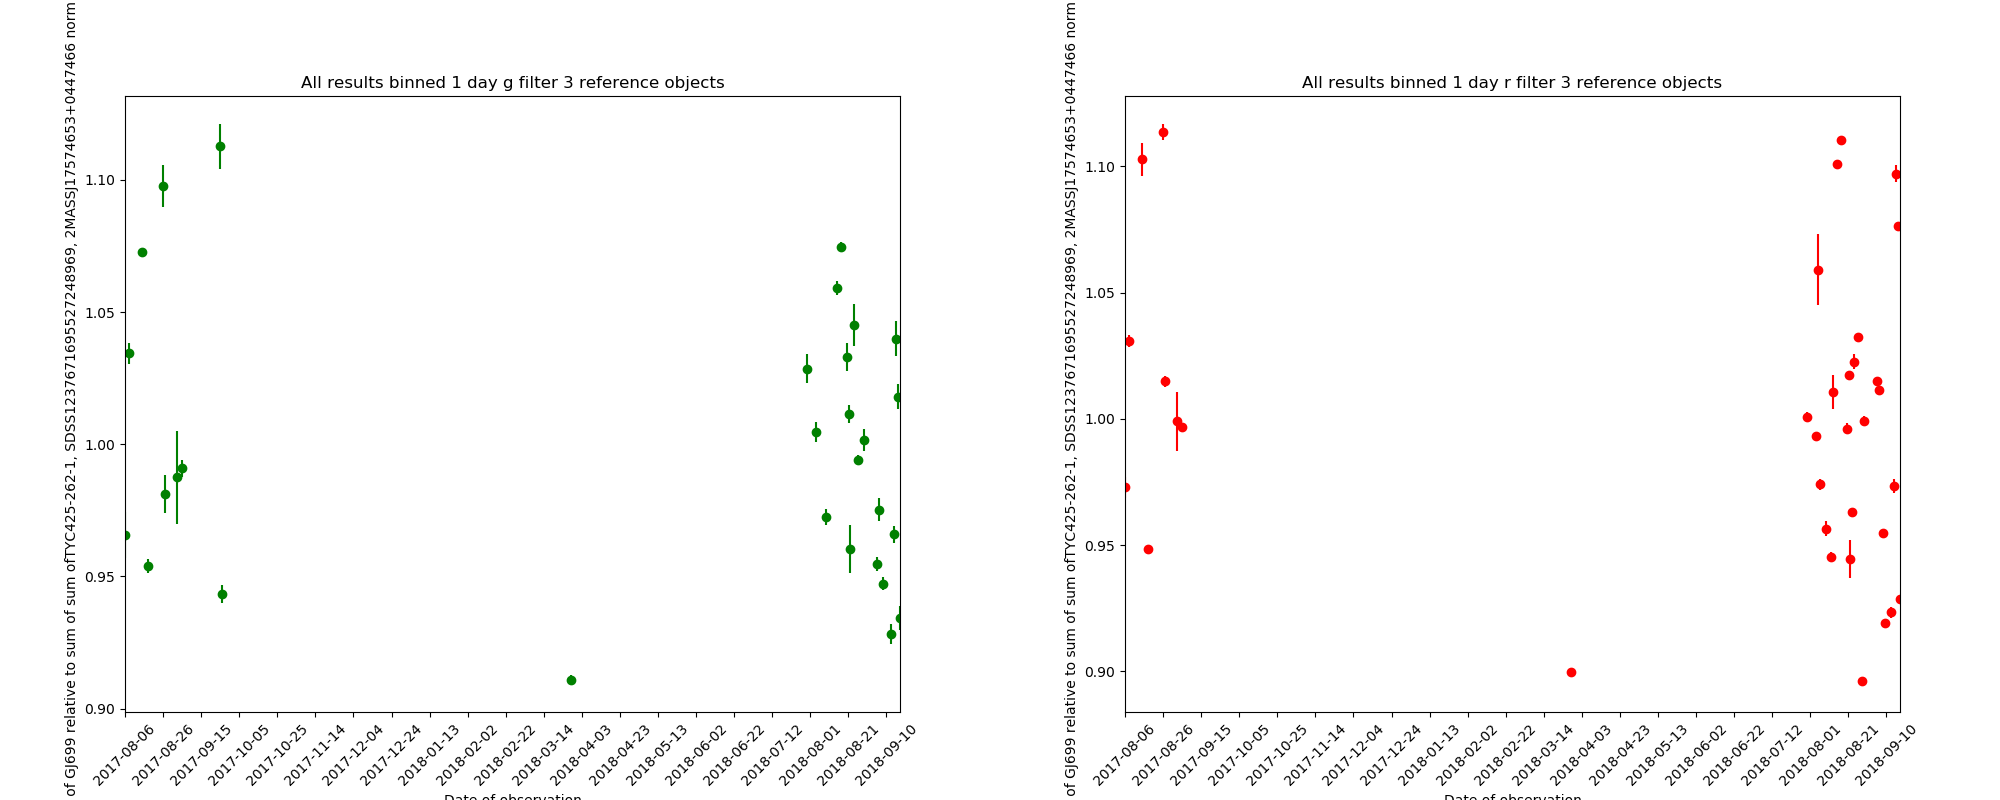
\includegraphics[scale=0.25]{images/allref123bin.png}
% \end{center}   
% \caption{This shows the ratio of the flux for the target, \bstar, to the 3 main reference objects as per Fig. \ref{fig:allref123} and binned to 1 day.}
%   \protect\label{fig:allref123bin}
% \end{figure}
% 
% \begin{figure}[!htbp]
% \begin{center}
% 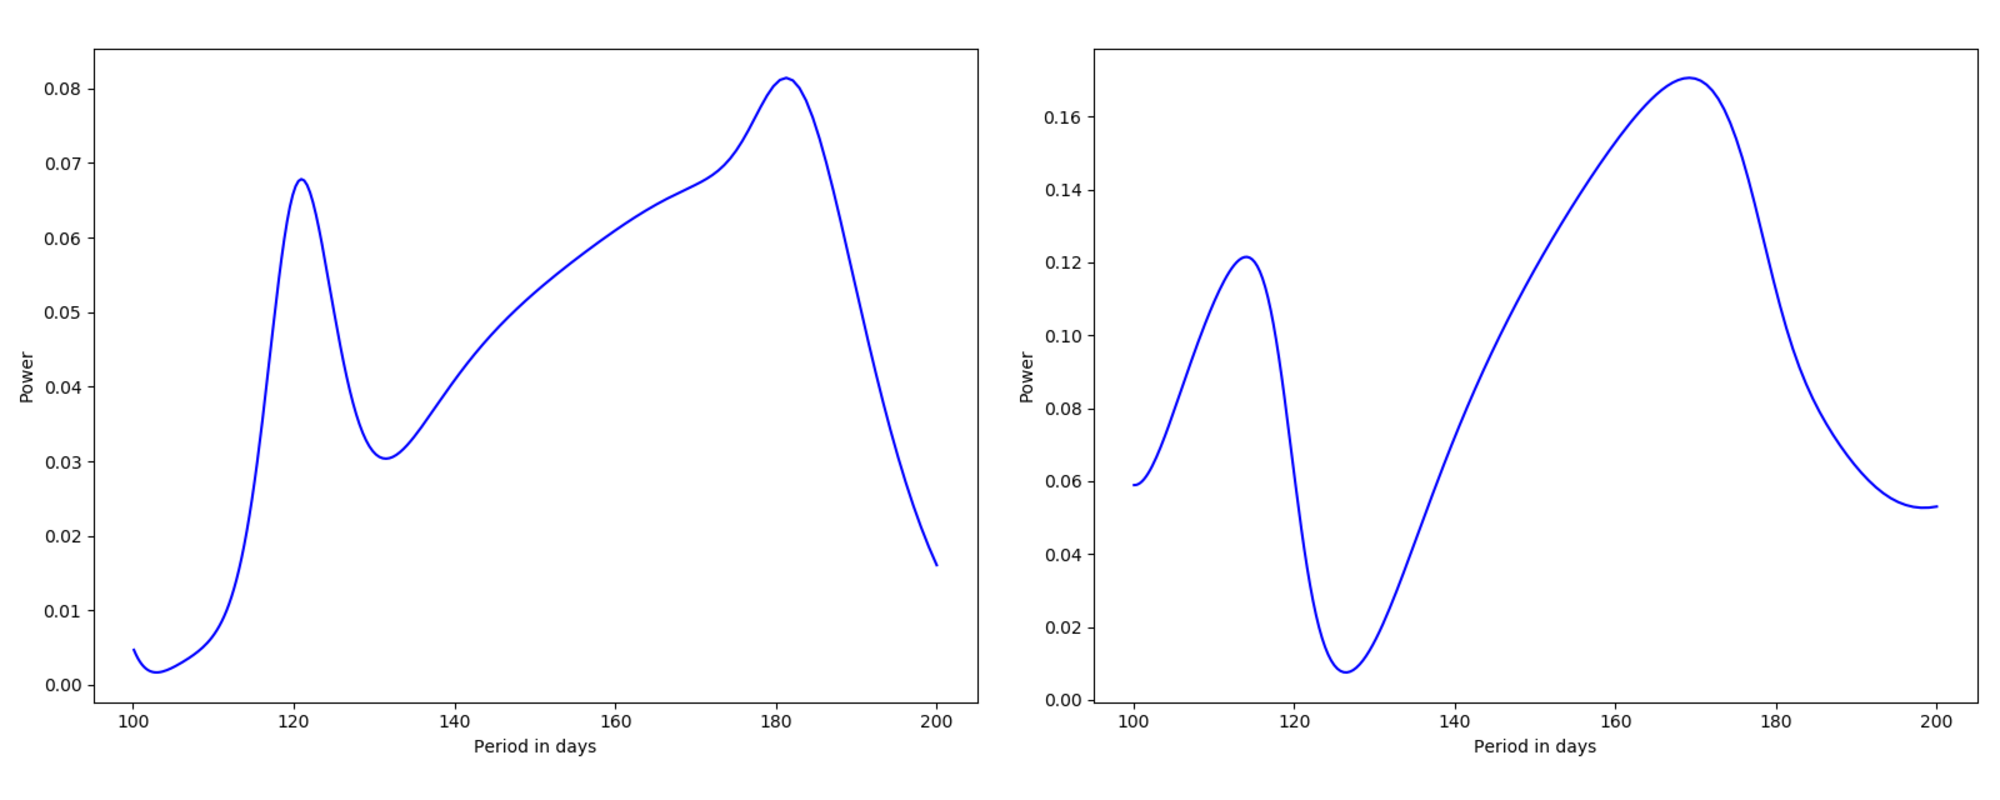
\includegraphics[scale=0.25]{images/ls123both.png}
% \end{center}   
% \caption{Periodograms obtained from Fig. \ref{fig:allref123}, left panel and Fig. \ref{fig:allref123bin} in right
%   panel. Only the \textbf{g} filter was used in this plot, the one from the \textbf{r} filter being almost identical.}
%   \protect\label{fig:ls123both}
% \end{figure}
% 
% \begin{figure}[!htbp]
% \begin{center}
% 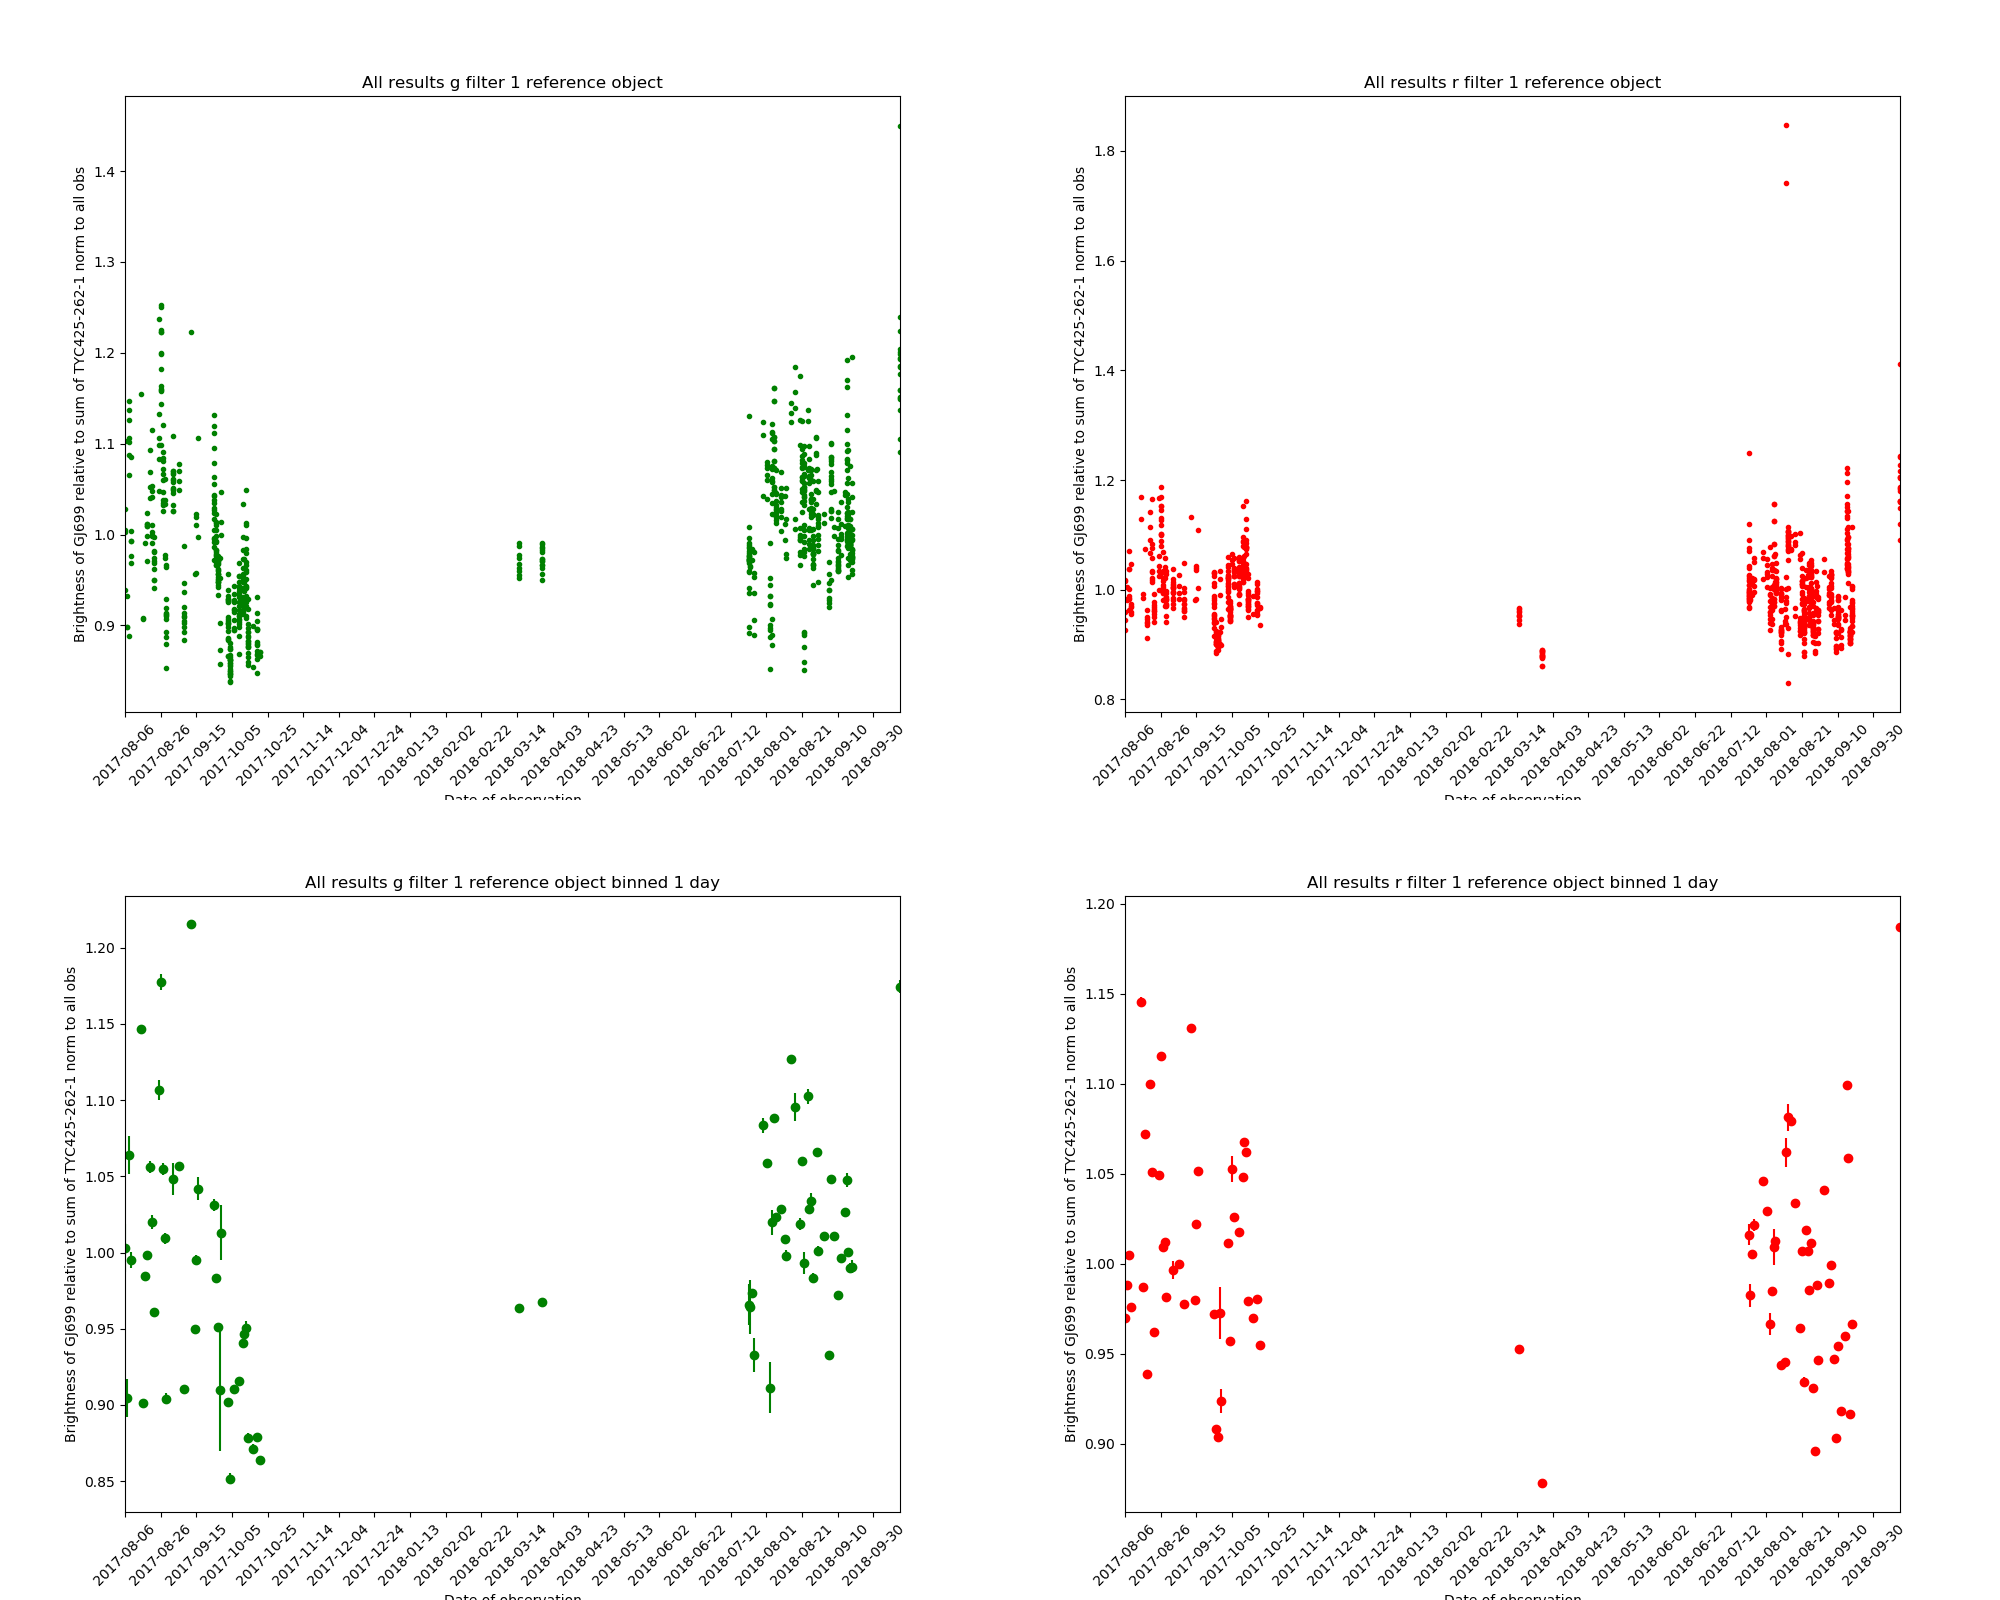
\includegraphics[scale=0.25]{images/allref1.png}
% \end{center}   
% \caption{This shows the ratio of the flux for the target, \bstar, to the strongest of the reference objects, TYC425-262-1.}
%   \protect\label{fig:allref1}
% \end{figure}
% 
% \begin{figure}[!htbp]
% \begin{center}
% 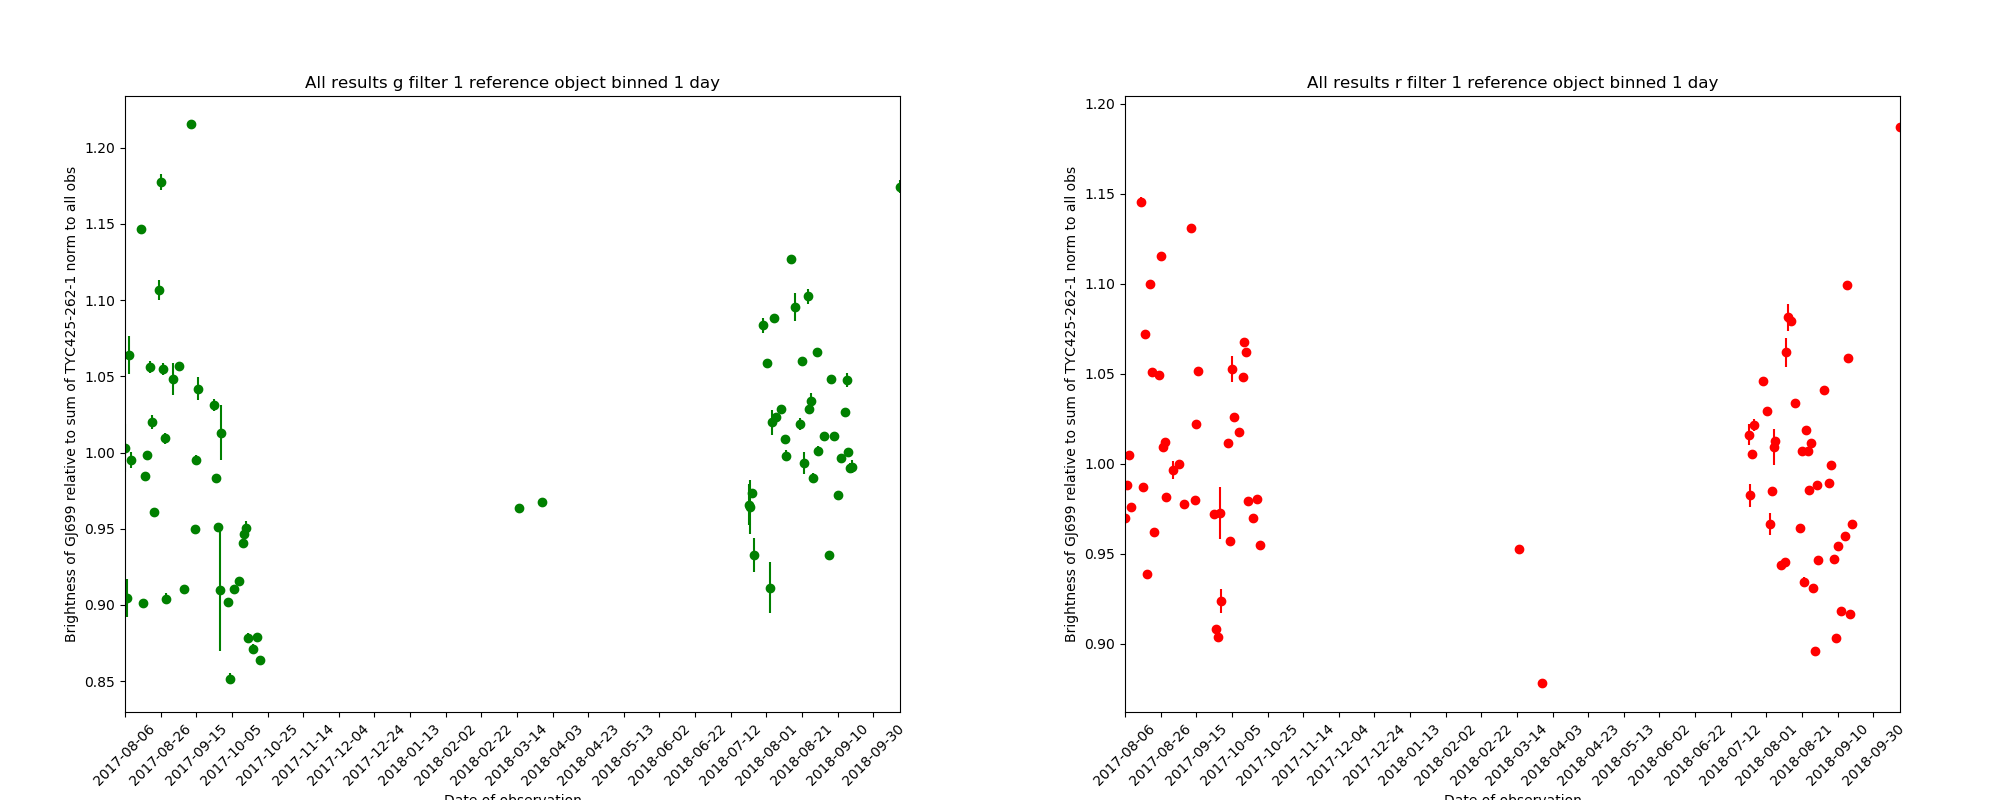
\includegraphics[scale=0.25]{images/allref1bin.png}
% \end{center}   
% \caption{This shows the ratio of the flux for the target, \bstar, to the strongest of the reference objects,
%   TYC425-262-1 per Fig. \ref{fig:allref1} and binned to 1 day.}
%   \protect\label{fig:allref1bin}
% \end{figure}
% 
% \begin{figure}[!htbp]
% \begin{center}
% 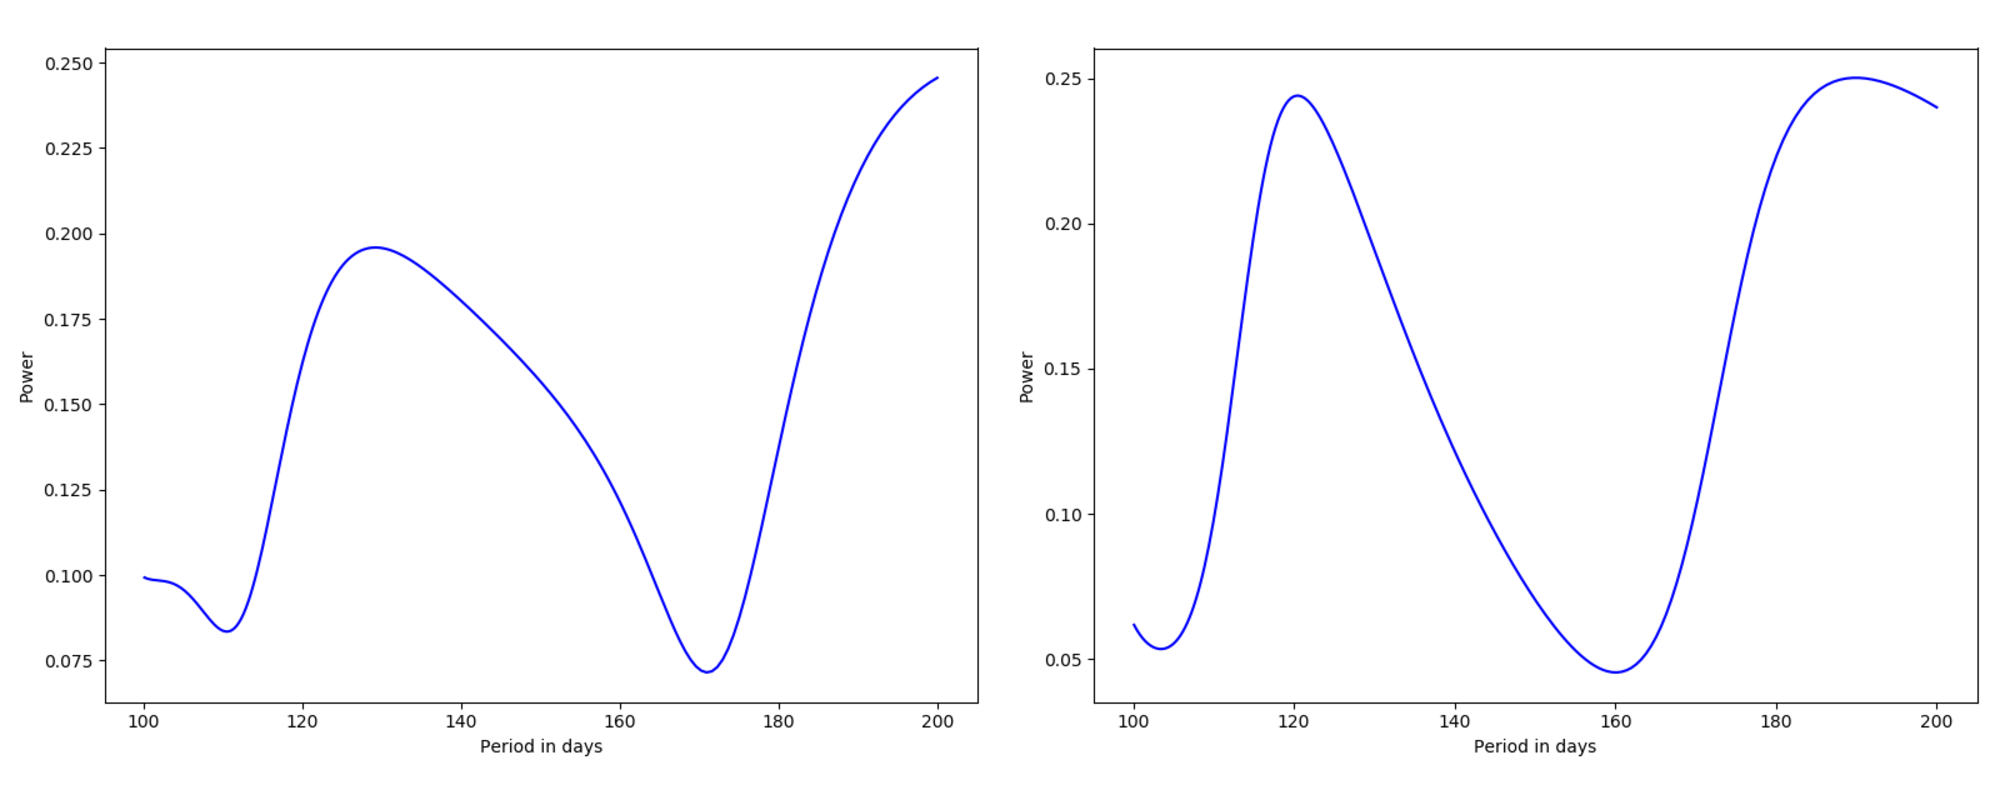
\includegraphics[scale=0.25]{images/ls1both.png}
% \end{center}   
% \caption{Periodograms obtained from Fig. \ref{fig:allref1}, left panel and Fig. \ref{fig:allref1bin} in right
%   panel. Only the \textbf{g} filter was used in this plot, the one from the \textbf{r} filter being almost identical.}
% \protect\label{fig:ls1both}
% \end{figure}
% \clearpage

